%%%%%%%%%%%%%%%%%%%%%%%%%%%%%%%%%%%%%%%%%%%%%%%%%%%%%%%%%%%
%% Congratulations, you've made an excellent choice
%% of writing your Tampere University thesis using
%% the LaTeX system. This document attempts to be
%% as complete a template as possible to let you focus
%% on the most important part: the writing itself.
%% Thus the details regarding the visual appearance
%% and even structure have already been worked out
%% for you!
%%
%% I sincerely hope you will find this template useful
%% in completing your thesis project. I've tried to
%% add comments (followed by the % sign) to clarify
%% the structure and purpose of some of the commands.
%% Most of the magic happens in the file tauthesis.cls,
%% which you are more than welcome to take a look at.
%% Just refrain from editing it in the most crucial
%% versions of the thesis!
%%
%% I wish you and your thesis project the best of luck!
%% If this template causes you trouble along the way
%% or if you've any suggestions for improving it,
%% please be in contact through GitHub
%% (<URL HERE>)
%%
%% Yours,
%%
%% Ville Koljonen
%%
%% PS. This template or its associated class file don't
%% come with a warranty. The content is provided as is,
%% without even the implied promise of fitness to the
%% mentioned purpose. You, as the author of the thesis,
%% are responsible for the entire work, including the
%% provided material. No one else is liable to you for
%% any damage inflicted on you or your thesis, were it
%% caused by using this template or not.
%%%%%%%%%%%%%%%%%%%%%%%%%%%%%%%%%%%%%%%%%%%%%%%%%%%%%%%%%%%

%%%%% NOTICE %%%%%
%% Please read through the entire template
%% (files under ./tex) to find all instructions.
%% It is possible that the attached pdf files
%% do not include the latest information.
%%%%%%%%%%%%%%%%%%

%%%%% INSTRUCTIONS FOR COMPILING THE DOCUMENT %%%%%
%% Overleaf: just click Recompile.
%% Terminal:
%%  1. pdflatex main.tex
%%  2. makeindex -s main.ist -t main.glg -o main.gls main.glo
%%  3. biber main
%%  4. pdflatex main.tex
%%  5. pdflatex main.tex
%% Similar sequence of commands is also required
%% in LaTeX specific editors.
%%%%%%%%%%%%%%%%%%%%%%%%%%%%%%%%%%%%%%%%%%%%%%%%%%%

%%% Set PDF version before doing anything else.

%%% set-pdf-version.tex
%
% This file is loaded by main.tex before any other operations, so that PDF
% version is set correctly for accessibility features.
%

\RequirePackage{ifluatex}

\def\mypdfminorversion{6}

\ifluatex

    \directlua {
        if pdf.getminorversion() \string~= \mypdfminorversion then
            if (status.pdf_gone and status.pdf_gone > 0)
            or (status.pdf_ptr and status.pdf_ptr > 0)
            then
                tex.error("PDF version cannot be changed anymore.")
            else
                pdf.setminorversion(\mypdfminorversion)
            end
        end
    }

\else

    \pdfminorversion=\mypdfminorversion

\fi


%%%%% METADATA %%%%%
%
% Always keep the following metadata up to date! This is important for your
% PDF file to comply to accessibility standards. (And yes, this information
% must remain here, before \documentclass[...]{...}.)

\def\myfititle{Piiloon jäävän syvyyden estimointi stereokuvista}
\def\myentitle{Estimating real depth data}
\def\myauthor{Esko Takku}
\def\myfisubtitle{Stereosyvyysdatan sekä segmentointidatasetin yhdistäminen puhtaan syvyyskartan generointiin}
\def\myensubtitle{Using stereo depth data and semantic segmentation dataset for generating a clean depthmap}
\def\myfithesistype{Diplomityö}
\def\myenthesistype{Masters Thesis}
\def\myexaminers{Joni Kämäräinen}
\def\myfifacultyname{Informaatioteknologian ja viestinnän tiedekunta}
\def\myenfacultyname{Faculty of Information Technology and Communication Sciences}
\def\myfiprogrammename{Tietotekniikka}
\def\myenprogrammename{Computer Sciences}
\def\myfikeywords{Stereonäkö, syvyysdata, semanttinen segmentointi}
\def\myenkeywords{Stereo vision, depth data, semantic segmentation}
\def\mylanguagecode{fi-FI}
\def\mysubject{Combining depth and segmentation data for real depthmap estimation}
\def\myyear{2025}
\def\mymonth{02}
\def\myday{23}

% Define your citation options here. Valid values for style and sorting options
% can be found in the BibLaTeX manual: https://ctan.org/pkg/biblatex.

\def\mycitationstyle{numeric}
\def\mycitationsorting{nyt}

%%%%% PREAMBLE %%%%%

%%%%% Document class declaration.
%
% The possible optional arguments are
%
%   finnish - thesis in Finnish (default)
%   english - thesis in English
%   draft - for faster non-final works, also skips images
%           (recommended, remove in final version)
%   programs - if you wish to display code snippets
% Example: \documentclass[english, authoryear]{tauthesis}
%          thesis in English with author-year citations

\documentclass[finnish]{tauthesis}

%%% preamble.tex
%
% This file is for including LaTeX libraries or packages and defining your own
% commands.
%
% NOTE: The glossaries package loaded by tauthesis.cls throws a warning: No
% language module detected for 'finnish'. You can safely ignore this. All
% other warnings should be taken care of, before your thesis is submitted!

%%%%% Your packages.
%
% Before adding packages, see if they can be found in tauthesis.cls already.
% If you're not sure that you need a certain package, don't include it in the
% document! This can dramatically reduce compilation time.

% Graphs
% \usepackage{pgfplots}
% \pgfplotsset{compat=1.15}

% Subfigures and wrapping text
% \usepackage{subcaption}

%% Theorem environments and their numbering.
%
% Define both English and Finnish theorem types. These all follow the same
% counter. See the documentation of amsthm to see how these can be changed to
% suit your needs, if necessary.
%

\usepackage{amsthm}

\theoremstyle{definition}

\newtheorem{definition}{Definition}[chapter]
\newtheorem{theorem}[definition]{Theorem}
\newtheorem{lemma}[definition]{Lemma}
\newtheorem{corollary}[definition]{Corollary}
\newtheorem{example}[definition]{Example}

\newtheorem{maaritelma}[definition]{Määritelmä}
\newtheorem{lause}[definition]{Lause}
\newtheorem{apulause}[definition]{Apulause}
\newtheorem{seurauslause}[definition]{Seurauslause}
\newtheorem{esimerkki}[definition]{Esimerkki}

% Mathematics packages
\usepackage{mathtools, amssymb}
%\usepackage{bm}

% Chemistry packages
% \usepackage{chemfig}
% \usepackage[version=4]{mhchem}

% Text hyperlinking
% \usepackage{hyperref}
% \hypersetup{hidelinks}

% (SI) unit handling
\usepackage{siunitx}

\sisetup{
    detect-all,
    math-sf=\mathrm,
    exponent-product=\cdot,
    output-decimal-marker={,} % for theses in FINNISH!
}

%% For code listings.

\usepackage{listings}

% This global code listing configuration is required for automatically
% replacing special characters with corresponding LaTeX commands, in code files
% included with \lstinputlisting. Without it, letters like 'ä' in code file
% comments will result in a LaTeX errors.
%
% Source: https://tex.stackexchange.com/a/574950.

\lstset{
    inputencoding = utf8,  % Input encoding
    extendedchars = true,  % Extended ASCII
    literate      =        % Support additional characters
        {á}{{\'a}}1  {é}{{\'e}}1  {í}{{\'i}}1 {ó}{{\'o}}1  {ú}{{\'u}}1
        {Á}{{\'A}}1  {É}{{\'E}}1  {Í}{{\'I}}1 {Ó}{{\'O}}1  {Ú}{{\'U}}1
        {à}{{\`a}}1  {è}{{\`e}}1  {ì}{{\`i}}1 {ò}{{\`o}}1  {ù}{{\`u}}1
        {À}{{\`A}}1  {È}{{\`E}}1  {Ì}{{\`I}}1 {Ò}{{\`O}}1  {Ù}{{\`U}}1
        {ä}{{\"a}}1  {ë}{{\"e}}1  {ï}{{\"i}}1 {ö}{{\"o}}1  {ü}{{\"u}}1
        {Ä}{{\"A}}1  {Ë}{{\"E}}1  {Ï}{{\"I}}1 {Ö}{{\"O}}1  {Ü}{{\"U}}1
        {â}{{\^a}}1  {ê}{{\^e}}1  {î}{{\^i}}1 {ô}{{\^o}}1  {û}{{\^u}}1
        {Â}{{\^A}}1  {Ê}{{\^E}}1  {Î}{{\^I}}1 {Ô}{{\^O}}1  {Û}{{\^U}}1
        {œ}{{\oe}}1  {Œ}{{\OE}}1  {æ}{{\ae}}1 {Æ}{{\AE}}1  {ß}{{\ss}}1
        {ẞ}{{\SS}}1  {ç}{{\c{c}}}1 {Ç}{{\c{C}}}1 {ø}{{\o}}1  {Ø}{{\O}}1
        {å}{{\aa}}1  {Å}{{\AA}}1  {ã}{{\~a}}1  {õ}{{\~o}}1 {Ã}{{\~A}}1
        {Õ}{{\~O}}1  {ñ}{{\~n}}1  {Ñ}{{\~N}}1  {¿}{{?`}}1  {¡}{{!`}}1
        {°}{{\textdegree}}1 {º}{{\textordmasculine}}1 {ª}{{\textordfeminine}}1
        {£}{{\pounds}}1  {©}{{\copyright}}1  {®}{{\textregistered}}1
        {«}{{\guillemotleft}}1  {»}{{\guillemotright}}1  {Ð}{{\DH}}1  {ð}{{\dh}}1
        {Ý}{{\'Y}}1    {ý}{{\'y}}1    {Þ}{{\TH}}1    {þ}{{\th}}1    {Ă}{{\u{A}}}1
        {ă}{{\u{a}}}1  {Ą}{{\k{A}}}1  {ą}{{\k{a}}}1  {Ć}{{\'C}}1    {ć}{{\'c}}1
        {Č}{{\v{C}}}1  {č}{{\v{c}}}1  {Ď}{{\v{D}}}1  {ď}{{\v{d}}}1  {Đ}{{\DJ}}1
        {đ}{{\dj}}1    {Ė}{{\.{E}}}1  {ė}{{\.{e}}}1  {Ę}{{\k{E}}}1  {ę}{{\k{e}}}1
        {Ě}{{\v{E}}}1  {ě}{{\v{e}}}1  {Ğ}{{\u{G}}}1  {ğ}{{\u{g}}}1  {Ĩ}{{\~I}}1
        {ĩ}{{\~\i}}1   {Į}{{\k{I}}}1  {į}{{\k{i}}}1  {İ}{{\.{I}}}1  {ı}{{\i}}1
        {Ĺ}{{\'L}}1    {ĺ}{{\'l}}1    {Ľ}{{\v{L}}}1  {ľ}{{\v{l}}}1  {Ł}{{\L{}}}1
        {ł}{{\l{}}}1   {Ń}{{\'N}}1    {ń}{{\'n}}1    {Ň}{{\v{N}}}1  {ň}{{\v{n}}}1
        {Ő}{{\H{O}}}1  {ő}{{\H{o}}}1  {Ŕ}{{\'{R}}}1  {ŕ}{{\'{r}}}1  {Ř}{{\v{R}}}1
        {ř}{{\v{r}}}1  {Ś}{{\'S}}1    {ś}{{\'s}}1    {Ş}{{\c{S}}}1  {ş}{{\c{s}}}1
        {Š}{{\v{S}}}1  {š}{{\v{s}}}1  {Ť}{{\v{T}}}1  {ť}{{\v{t}}}1  {Ũ}{{\~U}}1
        {ũ}{{\~u}}1    {Ū}{{\={U}}}1  {ū}{{\={u}}}1  {Ů}{{\r{U}}}1  {ů}{{\r{u}}}1
        {Ű}{{\H{U}}}1  {ű}{{\H{u}}}1  {Ų}{{\k{U}}}1  {ų}{{\k{u}}}1  {Ź}{{\'Z}}1
        {ź}{{\'z}}1    {Ż}{{\.Z}}1    {ż}{{\.z}}1    {Ž}{{\v{Z}}}1
}

%%%%% Your commands.

% Print verbatim LaTeX commands
\newcommand{\verbcommand}[1]{\texttt{\textbackslash #1}}

% Command for formatting code.

\newcommand\code[1]{\texttt{#1}}

% A delimiter command for the norm of a vector with mathtools.

\DeclarePairedDelimiter\norm{\lVert}{\rVert}

% Basic theorems in Finnish and in English.
% Remove [chapter] if you wish a simply
% running enumeration.
% \newtheorem{lause}{Lause}[chapter]
% \newtheorem{theorem}[lause]{Theorem}

% \newtheorem{apulause}[lause]{Apulause}
% \newtheorem{lemma}[lause]{Lemma}

% Use these versions for individually
% enumerated lemmas
% \newtheorem{apulause}{Apulause}[chapter]
% \newtheorem{lemma}{Lemma}[chapter]

% Definition style
% \theoremstyle{definition}
% \newtheorem{maaritelma}{Määritelmä}[chapter]
% \newtheorem{definition}[maaritelma]{Definition}
% examples in this style

%%%%% Glossary information.

% Use the following lines ONLY if you need more
% than one glossary. The first argument specifies
% a type label for the glossary and the second
% the displayed name.
% \newglossary*{symbs}{Symbols}
% \newglossary{label}{Displayed name}
% ...

\makeglossaries

% Use this line if using the default glossary.
% Otherwise comment out.

\loadglsentries[main]{tex/sanasto.tex}

% Use this line if using more than one glossary.
% Otherwise comment out.
% \loadglsentries[symbs]{tex/sanasto2.tex}

%%%%% Citation information.

% Commonly used bibliography modifications.
% Feel free to play around with them.

%\ExecuteBibliographyOptions{%
%sorting=none,
%maxbibnames=99,
%maxcitenames=2,
%giveninits=true,
%uniquename=init,
%sortcites,
%sortlocale=fin}

%\DeclareNameAlias{sortname}{last-first}
%\DeclareNameAlias{author}{last-first}

%\DeclareFieldFormat[%
%    article,inbook,incollection,inproceedings,
%    patent,thesis,unpublished]{citetitle}{#1\isdot}
%\DeclareFieldFormat[%
%    article,inbook,incollection,inproceedings,
%    patent,thesis,unpublished]{title}{#1\isdot}
%\DeclareFieldFormat{pagetotal}{#1 \bibstring{page}}

%\AtBeginBibliography{\renewcommand*{\makelabel}[1]{#1\hss}}

%\DefineBibliographyExtras{english}{\let\finalandcomma=\empty}

\addbibresource{tex/references.bib}
 % You can add packages and define new commands in this file.

\begin{document}

%%%%% FRONT MATTER %%%%%

\frontmatter

%%%%% Thesis information and title page.

% Enable the use of @ character in command names.

\makeatletter

% The titles of the work. If there is no subtitle, leave the \myfisubtitle or
% \myensubtitle command arguments empty. Pass the title in the primary
% language as the first argument and its translation to the secondary language
% as the second.

\if@langenglish

    \title{\myentitle}{\myfititle}

\else

    \title{\myfititle}{\myentitle}

\fi

\if@langenglish

    \subtitle{\myensubtitle}{\myfisubtitle}

\else

    \subtitle{\myfisubtitle}{\myensubtitle}

\fi

% The author name.

\author{\myauthor}

% The examiner information. If your work has multiple examiners, replace with
%
%   \examiner[<label>]{<name> \\ <name>}
%
% where <label> is an appropriate (plural) label, e.g. Examiners or
% Tarkastajat, and <name>s are replaced by the examiner names, each on their
% separate line.

\examiner{\myexaminers}

% The finishing date of the thesis (YYYY-MM-DD).

\finishdate{\myyear}{\mymonth}{\myday}

% The type of the thesis (e.g. Kandidaatintyö or Master of Science Thesis) in
% the primary and the secondary languages of the thesis.

\if@langenglish

    \thesistype{\myenthesistype}{\myfithesistype}

\else

    \thesistype{\myfithesistype}{\myenthesistype}

\fi

% The faculty and degree programme names in the primary and the secondary
% languages of the thesis, respectively.

\if@langenglish

    \facultyname{\myenfacultyname}{\myfifacultyname}

\else

    \facultyname{\myfifacultyname}{\myenfacultyname}

\fi

\if@langenglish

    \programmename{\myenprogrammename}{\myfiprogrammename}

\else

    \programmename{\myfiprogrammename}{\myenprogrammename}

\fi

% The keywords of the thesis in the primary and the secondary languages of the
% thesis.

\if@langenglish

    \keywords{\myenkeywords}{\myfikeywords}

\else

    \keywords{\myfikeywords}{\myenkeywords}
\fi

% Make @ a regular letter again.

\makeatother

% Actually generate the title page based on the above commands.

\maketitle


%%%%% Abstracts and preface.
%
% Write the abstract(s) and the preface into a separate file for the sake of
% clarity. Pass the appropriate file name as the first argument to these
% commands. Put the \abstract in the primary language first and the
% \otherabstract in the secondary language second. Those who do not speak
% Finnish only need the first abstract. The second argument of the \preface
% command takes the place where the thesis was signed in.

\abstract{tex/tiivistelma.tex}

\otherabstract{tex/abstract.tex}

\preface{tex/alkusanat.tex}{Tampereella}

%%%%% Table of contents.

\tableofcontents

%%%%% Lists of figures, tables, listings and terms.
%
% Print the lists of figures and/or tables. Uncomment either of these commands
% as required. Both are optional, but if there are many important
% figures/tables, listing them may be a good idea.

% \listoffigures
% \listoftables
% \lstlistoflistings

% Misc stuff related to how the glossary is displayed. You can especially
% tweak the lengths to suit you!

\glsaddall
\setglossarystyle{taulong}
\setlength{\glsnamewidth}{0.25\textwidth}
\setlength{\glsdescwidth}{0.75\textwidth}
\renewcommand*{\glsgroupskip}{}

% Print the default glossary of abbreviations, if necessary. Otherwise comment
% out. The appropriate Finnish variant is 'Lyhenteet'

\printglossary[title={Lyhenteet ja merkinnät}]

% Print more than one glossary with these lines. Otherwise comment out.

% \printglossary[type=symbs]
% \printglossary[type=label]
% ...

%%%%% MAIN MATTER %%%%%

\mainmatter

% Write each of the chapters of the thesis into a separate file for the sake
% of clarity. They can be \input as shown below. Give both the chapters and
% their files as descriptive names as possible.

\chapter{Johdanto}%
\label{ch:johdanto}

Koneoppimisella voidaan hakea ratkaisua monenlaisiin ongelmiin. Sen avulla voidaan pyrkiä ratkaisemaan normaalisti erittäin monimutkaisia algoritmeja vaativia ongelmia. Käytännössä mikä tahansa tietotekninen ongelma on teoriassa ratkaistavissa koneoppimisella. Se ei kuitenkaan aina ole tarpeellinen tai mahdollinen ratkaisu. Tarpeettoman monimutkaisuuden sekä ”black box” ongelmien välttelyn ohella, yhtenä suurimpana esteenä sen toteuttamisessa on hyvän koulutusdatan hankkiminen. Tämänhetkiset käyttökelpoiset mallit koulutetaan koulutusdatan avulla, ja nämä mallit voivat olla vain yhtä hyviä kuin niissä käytettävä koulutusdata.

Näin ollen jos halutaan luoda malli joka ei käytä yleisesti saatavilla olevaa koulutusdataa, hankaloituu sen luominen huomattavasti. Yleisimmin saatavilla olevat mallit ovat ihmisten sekä asioiden tunnistamiseen. Jos tavoittelemamme asia on variaatio tästä tai jostain muusta yleisestä mallista, voi uuden datan luomiseen alusta aloittamisen sijaan käyttää olemassa olevia malleja. Kuitenkin mitä kauemmas siirrytään selkeästä tehtävästä niin kuin objektin tunnistus, hankaloituu totuuden määrittäminen ja näin ollen myös hyvän ja toimivan mallin luominen.

Tässä työssä pyritään käyttämään segmentointi sekä syvyysdataa mallin luomiseen joka antaa syvyysdatan, ilman liikkuvia kohteita niin kuin autoja tai ihmisiä. Tämä pyritään saavuttamaan mahdollisimman automaattisesti, ja tavalla joka on hyödynnettävissä mahdollisimman geneerisesti eri mallien kanssa.

Lopullisen koulutusdatan generointiin tarvitaan siis tieto irtonaisista kohteista kuvassa, kuvan syvyysdata sekä jonkinlainen arvio tunnistetun kohteen takana olevasta alueesta. Paras keino tämän datan generointiin olisi kuvien manuaalinen läpikäynti ja syvyysdatan ”värittäminen” kuvaan. Tässä työssä kuitenkin pyritään työ tekemään mahdollisimman automaattisesti, resurssien säästämiseksi. Vaikka datan generointiin voidaankin käyttää pitkälti perinteisiä kuvankäsittely algoritmeja ei sen avulla todennäköisesti ole mahdollista tuottaa täysin luotettavaa dataa, koska kohteiden takana olevien asioiden tieto puuttuu stereokuvista. Tämän tiedon irrottaminen automaattisesti voisi olla mahdollista jos lähtökohtana käytettäisiin videokuvaa, mutta toteutettavan mallin kompleksisuus kasvaisi huomattavasti. Datasetin luominen alusta olisi myös mahdollista jos stereokameralla otettaisiin kuvia samasta kohteesta niin pitkällä aikavälillä että kaikki liikkuvat kohteet olisivat väistyneet. Tällaisen datasetin luominen tai löytäminen on kuitenkin hyvin hankalaa. 

Tällaista mallia voisi pidemmälle jalostettuna hyödyntää moniin eri käyttökohteisiin. Sitä voisi hyödyntää automatisoinnissa, kun tilasta saadaan helposti puhdas malli. Näin voidaan generoida esimerkiksi automaattiajamisessa käytettävät liikkeet suoraan tyhjään tilaan. Samaa voisi hyödyntää tilojen 3d skannauksessa. Ei olisi niin tarpeellista siivota tilaa ja jatkojalostuksella tunnistetut huonekalut tai muut siirrettävät asiat voitaisiin sisustaa suoraan generoituun pistepilveen tai 3d malliin. Tämä mahdollistaisi myös 3d skannauksen esimerkiksi peleissä, jolloin ympäristö voisi olla suoraan interaktiivinen, ilman niin suurta manuaalista työtä. 

Tässä työssä käytettävä data on itseajavien autojen kehitykseen liittyvää kaupunkidataa. Siitä löytyy valmiina, syvyysdata sekä segmentointidata. Kuitenkin koska mallin ja sen rakentamistyökalujen tulee olla hyödynnettävissä myös muulla datalla, käydään läpi myös stereokuvasta syvyysdatan hankinta, sekä segmentointimallin luonti. Lopputuloksessa käytetään kuitenkin, valmiiksi tarjottuja malleja segmentoinnin sekä syvyysdatan osalta.

Lopullisen tuotoksen olisi tarkoitus olla malli jolle tarjotaan stereokuva ja se palauttaa syvyysdatan ilman liikkuvia kohteita kuvassa.

\chapter{Kirjallisuuskatsaus}%
\label{ch:Kirjallisuuskatsaus}

Kirjoita tähän sellainen

\chapter{Teoria}%
\label{ch:teoria}

\section{Stereoanalyysi}

Stereoanalyysi kuvankäsittelyssä tarkoitetta kahdesta samasta kohteesta otetusta kuvasta olevien yhtenäisyyksillä syvyyden analysointia.
Vaikka näitä tekniikoita voi soveltaa mihin tahansa kuviin jotka ovat samasta kohteesta \cite{SumiYasushi20023ORi},
tässä yhteydessä käytämme kuvia,
jotka ovat otettu samasta perspektiivistä siten että kuvat ovat horisontaalisesti vierekkäin.
Jos tiedetään kameroiden suhteelliset sijainnit tai jonkin pisteen etäisyys kamerasta voidaan myös kuvasta arvioida absoluuttinen etäisyys kameraan. 

\begin{figure}[h]
\centering
\pdftooltip{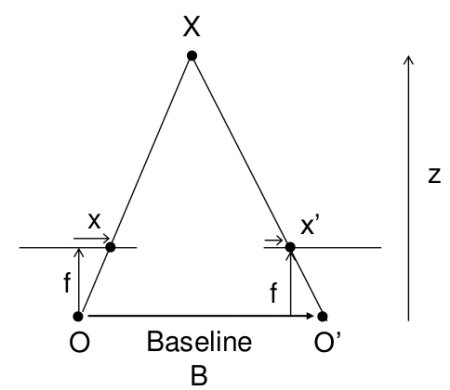
\includegraphics[width=\textwidth]{figures/stereo_depth.jpg}}{Stereo depth}
\caption{Stereo syvyyden arviointi}
\label{fig:stereo}
\end{figure}
    
Kun stereoparia analysoidaan ja tunnistetaan korreloiva piste molemmista kuvista,
voidaan laskea kuvien välinen dispariteetti Kuva \ref{fig:stereo}
Tämä tarkoittaa käytännöstä muutosta pisteen sijainnissa kuvien välillä.
Periaatteessa vastaavat pisteet voivat sijaita missä tahansa kuvassa.
Kuitenkin tässä tapauksessa jossa kuvat ovat tietyssä suhteessa toisiinsa,
voidaan olettaa stereoparin löytyvän x-akselilta tai ainakin melko läheltä sitä.
Jos näin ei olisi jouduttaisiin kuvan jokaista pistettä vertaamaan jokaiseen pisteeseen toisessa kuvassa.
Tämä tapa tulee nopeasti laskennallisesti hyvin kalliiksi.
Jos verrattava alue on myös hyvin pieni todennäköisyys tunnistaa useita samankaltaisia alueita kasvaa.
Jos alue on suuri tai vertailu suoritetaan liian tarkasti,
kasvaa todennäköisyys että vaihtunut kuvakulma on niin erilainen että sitä ei tunnisteta.
Tästä johtuen tämän ongelman ratkaisuun on kehitetty monia erilaisia tapoja.


\subsection{SGM - Semi Global Matching}

Jotta stereoanalyysi on mahdollista,
tulee kuvasta tunnistaa samat kohteet.
Yksi tapa tehdä tämä on Hircmullerin SGM tekniikalla \cite{hirschmuller2005babel}.
Tämä tekniikka ottaa huomioon pikselin ja sen ympäröivien pikselien arvot etsiessään toisesta kuvasta vastaavaa arvoa. Tämä haku voidaan tehdä kaavalla.

\begin{equation}\label{yht:SGM}
    E(d) = \sum_{p} D(p, d_p) + \sum_{q \in \mathcal{N}} R(p, d_p, q, d_q)
\end{equation}

Kaavassa \(D(p, d_p)\) summafunktio käy läpi kaikki kuvan pikselit ja vertaa niitä vertailupikseliin.
Tämä antaa perusarvon yksittäisen pikselin samankaltaisuudelle.

Tämän jälkeen pikselin ympäröiviä pikseleitä verrataan toisiinsa \(R(p, d_p, q, d_q)\).
Koska samaa asiaa ympäröivien pikselien tulisi olla samankaltaisia molemmissa kuvissa,
vaikka ne onkin kuvattu hieman eri asennosta, voidaan tämän avulla arvioida onko kyseessä sama piste.

Tämän algoritmin toteuttaa pythonin opencv kirjaston SGBM \cite{opencvsgbm},
jota muokattu alkuperäiseen toteuytukseen verrattuna käymään läpi pikselijoukkoja, eikä yksittäisiä pikseleitä.
Tämä nopeuttaa prosessointia huomattavasti \cite{MemoryEfficientSGM}.

\section{Neuroverkot} 

Tämän työn lopputulos on neuroverkko.
neuroverkko on yleisesti kuva-analyysiin sekä muuhun koneoppimiseen käytettävä tekniikka.
Sen toiminta perustuu neuroneihin joita järjestetään verkkomaiseen rakenteeseen useisiin eri kerroksiin.
Sen lähtökohta on ihmisaivojen toiminnan matkiminen joka on nykyisen koneoppimistekniikan perusta \cite{PhamTrungQuang2023EotH}.


\begin{equation}\label{yht:neuroni}
    a = \sigma\left(\sum_i w_i x_i + b\right)
\end{equation}

Tämä on neuronin matemaattinen kaava,
se tuottaa ulostulonaan arvon \(a\) saamiensa syötteiden perusteella.
\(x_i\) on neuronin saama syöte.
\(w_i\) on neuronille annettu painoarvo.
\(b\) on neuronin harha arvo. \(\sigma\) on funktio joka muuttaa neuronin saavan armon välille 0,1.


Neuroverkko on siis vain joukko yksinkertaisia matemaattisia funktioita,
joiden toimintaa muokkaamalla pyritään saamaan haluttu lopputulos.
Jotta lopputulos on koskaan haluttu pitää tätä koulutusprosessia kuitenkin valvoa.


Kun näitä neuroneita asetetaan eri kerroksiin siten että verkon sisääntulo on esimerkiksi valokuvan kokoinen, 
ja ulostulo on yhen neuronin ulostulo, 
voidaan verkolle syöttää kuvia esimerkiksi kissoista ja koirista.
Kun näille kuville annetaan arvot 0 ja 1 kuvan aiheen mukaan, voidaan verkko kouluttaa tunnistamaan kissoja ja koiria.
Koulutuksen aikana verkko muuttaa arvojaan \(w_i\) ja \(b\).
Nämä arvot se saa yrittämällä erilaisia arvoja neuroneille.
Kun verkkoa tämän jälkeen testataan on voidaan saaduista lopputuloksista valita paras.
Tämän jälkeen tätä lopputulosta voidaan lähteä parantelemaan, testaamalla toimiiko suuremmat vai pienemmät arvot paremmin.
Kun näitä kahta arvoa eri neuroneilla muutetaan voidaan saada paremmin toimiva neuroverkko.
Tarpeeksi monen yrityksen jälkeen, saadaan siis todennäköisesti verkko joka tunnistaa onko kuvassa todennäköisemmin kissa vai koira

Tätä satunnaisuutta pyritään siis parantamaan ohjaamalla verkon koulutusta.
Tämä tapahtuu tappiofunktion (loss function) sekä takaisinvirtausalgoritmin (backpopagation algorithm) avulla.

Tappiofunktion tehtävä on kertoa kuinka paljon saatu tulos eroaa halutusta.
Esimerkkitapauksessamme tämä käytännössä testaa, verkon lopputuloksen ja palauttaa kuinka monta arvausta verkko sai oikein,
tämä käytännössä katsoisi onko verkolle annetun kissa kuvan ulostulon arvo mikä sen pitäisi olla.
Virheen tunnistus ei kuitenkaan ole aina yhtä yksinkertaista, tämän työn lopputulos on verkko joka yrittää luoda kuvasta 3d pistekartan.
Siinä tapauksessa siis neliösumma tai jokin muu tapa virheen tunnistamiseen olisi parempi.
Kun virhe on tunnistettu verkkoa muokataan takaisinvirtaus algoritmin perusteella.
Näihin algoritmeihin ei ole yhtä parasta ratkaisua, vaan eri verkkojen ja käyttökohteiden tapauksessa eri algoritmit voivat tuoda hyvin erilaisia tuloksia.

\section{Semantic segmentation}

Semantic segmentation eli kuvan segmentointi on yleinen käyttökohde neuroverkoille.
Sen avulla on helppo tehdä käytettäviä ja helposti hyödynnettäviä malleja.
Ja se on hyvä esimerkki ongelmasta jolle on helppo tehdä koulutusdataa, mutta hankala luoda ohjelmallista toteutusta saman lopputuloksen saamiseksi.
Esimerkkejä käytöstä on esimerkiksi automatisoidussa liikenteessä esteiden tunnistuksessa Kuva \ref{fig:labels}.

\begin{figure}[h]
\centering
\pdftooltip{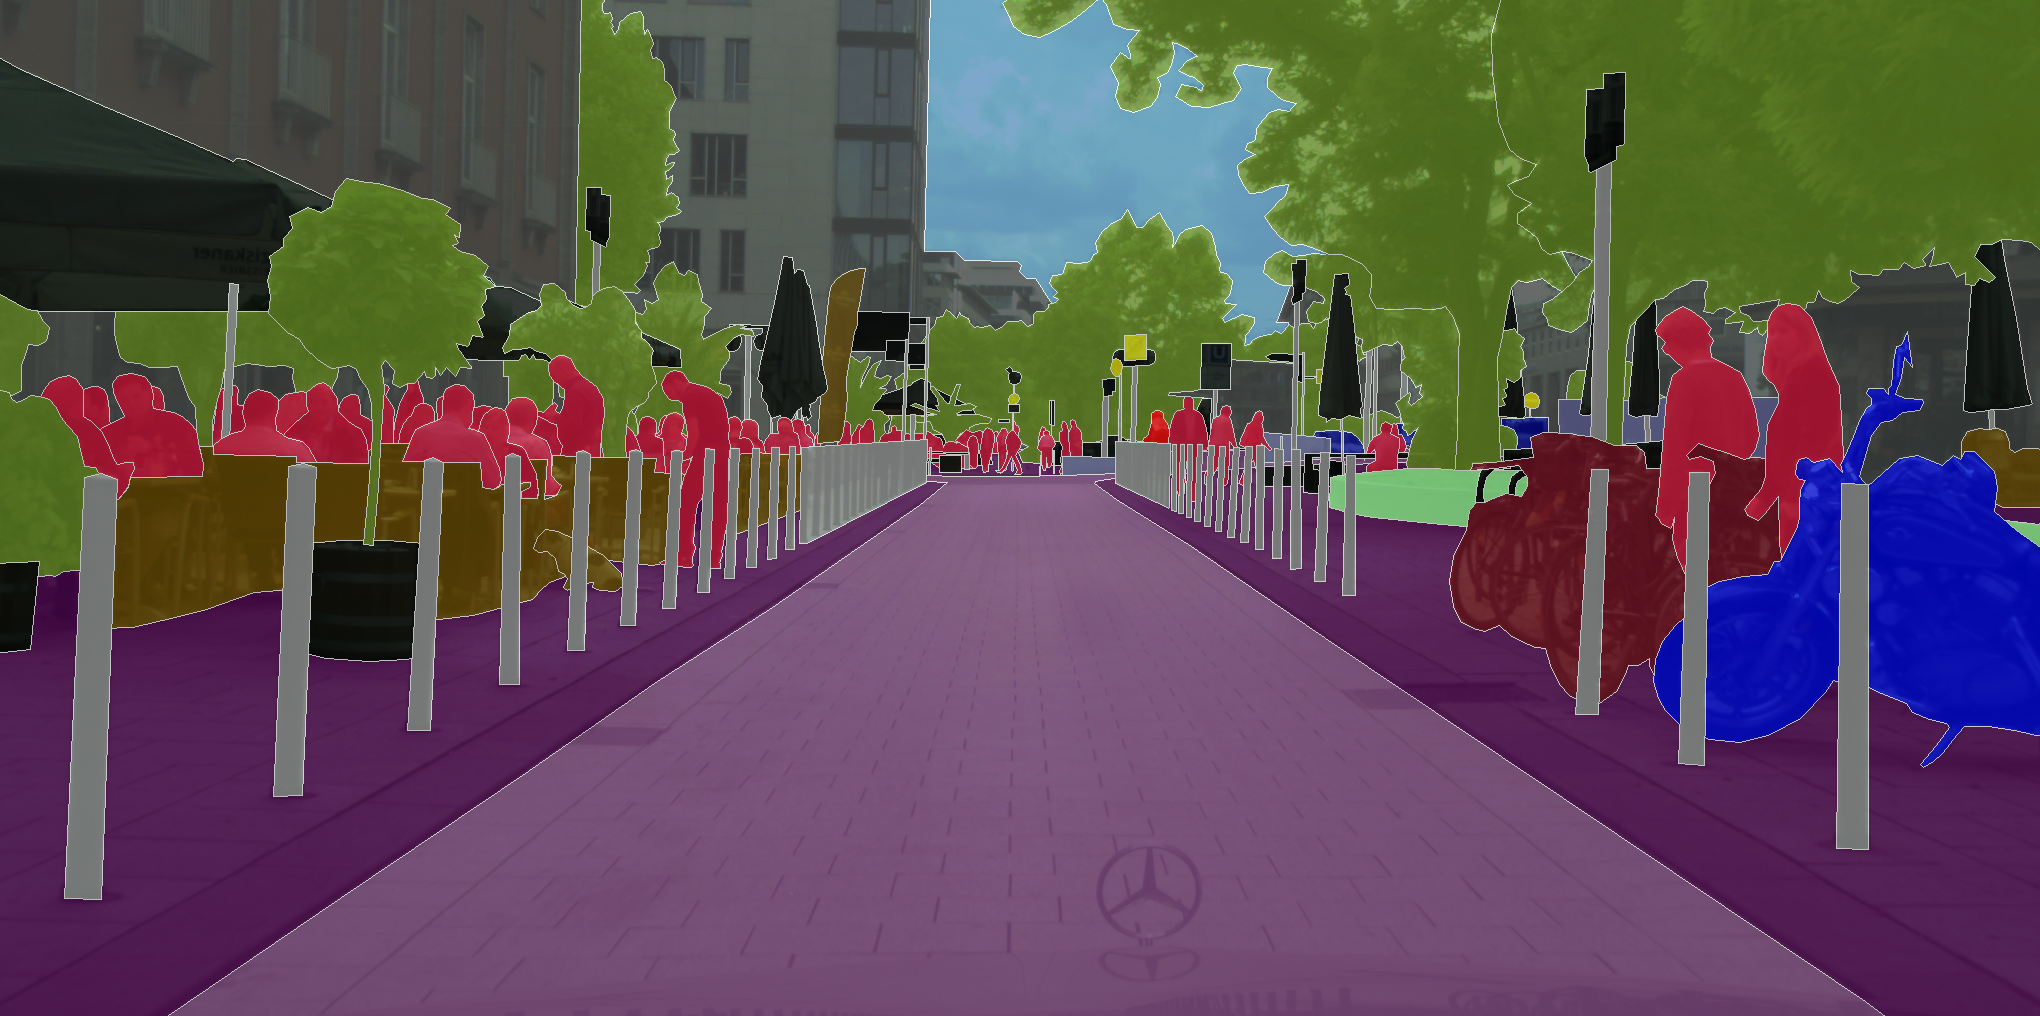
\includegraphics[width=\textwidth]{figures/stuttgart03.png}}{Cityscapes esimerkki kuva stuttgart03}
\caption[Tämä on lyhyt kuvateksti.]{Cityscapes datestin esimerkki segmentointi dataa, jossa kaupunkinäkymän erilaiset tunnistattavat kohteet on merkitty eri väreillä.}
\label{fig:labels}
\end{figure}

Tätä teknologiaa voidaan soveltaa useiden eri tunnistusongelmien ratkaisuun.
Koulutusdatasta riippuen kuvasta voidaan tunnistaa mitä tahansa.
Samaa teknologiaa käytetään teollisissa sovellutuksissa laadunvalvonnassa,
sekä lääketieteessä erilaisten skannausten analysoinnissa \cite{NagalakshmiT2022BCSS}.
Mallin voi kouluttaa tunnistamaan useita tai vain yhtä asiaa riippuen käyttökohteesta.
Toisin kuin perinteinen tunnistusmalli, joka tunnista yleensä vain mitä kuvassa on,
segmnetaatiomalli antaa joka pikselille arvon jonka perusteella lopputuloksesta voidaan nähdä, mitä eri kohdissa kuvaa on.
Jotta samanlainen lopputulos saataisiin kohteentunnistusmallilla pitäisi kuvaa käydä läpi pienemmissä lohkoissa jotta rajat löytyisivät.
Kohteen tunnistusta voisi myös hyödyntää eri kohteiden etäisyyden arviointiin, jota voisi hyödyntää niiden takana olevan syvyyden arvioimiseen \cite{ShiZhou2023VRBo}.

Segmentointimallin kouluttaminen ja datasetin käsittely on hieman haastavampaa kuin kohteentunnistusmallin.
Jotta mallin voi kouluttaa tunnistamaan asiat pikselitasolla, on myös opetusdatan oltava pikselitasolla määriteltyä. 
Myöskin datan koulutuksessa käytettävä tappiofunktion määrittely hieman hankaloituu.
Mallin koulutuksessa pitää käyttää jotain muuta tapaa tunnistaa sen onnistuminen, kuin vain ”onko kyseessä auto”.

Yksi segmentointimallin koulutuksessa käytettävä tappion laskutapa, 
jota myös tässä työssä käytetään, on ristientropian virhefunktio (Cross Entropy Loss) \cite{CrossEntropyLoss}. 

Ristientoripa virhefunktio vertaa mallin tuottamia toednnäköisyyksiä oikeaan malliin. 
Sille lasketaan virhe ottamalla negatiivinen logaritmi oikeaan luokkaan liittyvästä todennäköisyydestä ja lisäämällä sen arvo kaikkien havaintojen yli.
Tämä siis tarkoittee, että mallin ennustaman todennäköisyyden ja todellisen luokan välille lasketaan epävarmuus jonka avulla mallia voidaan ohjata oikeaan suuntaan.
Mitä enemmän alueet osuvat oikeaan, sitä pienemmäksi mallin virhe laskee.

\section{Syvyyskartta}

Tämän työn haluttu lopputulos on syvyyskartta \cite{IkeuchiKatsushi1987DaDM}.
Syvyyskartta on yksinkertainen kuvan kaltainen esitystapa, jossa eri syvyyksillä on eri numeerinen arvo.
Se voidaan näyttää esimerkiksi siten että kauempana kamerasta oleva kohde on tummemmalla värillä \ref{fig:depth}.
Tärkeä ero 3d-malliin sekä syvyyskartan välillä on datan perspektiivi.
Syvyyskartassa ei ole tietoa kohteiden takana olevasta tilasta, joten sitä voi tarkastella vain sen kuvaus perspektiivistä.


\begin{figure}[h]
\centering
\pdftooltip{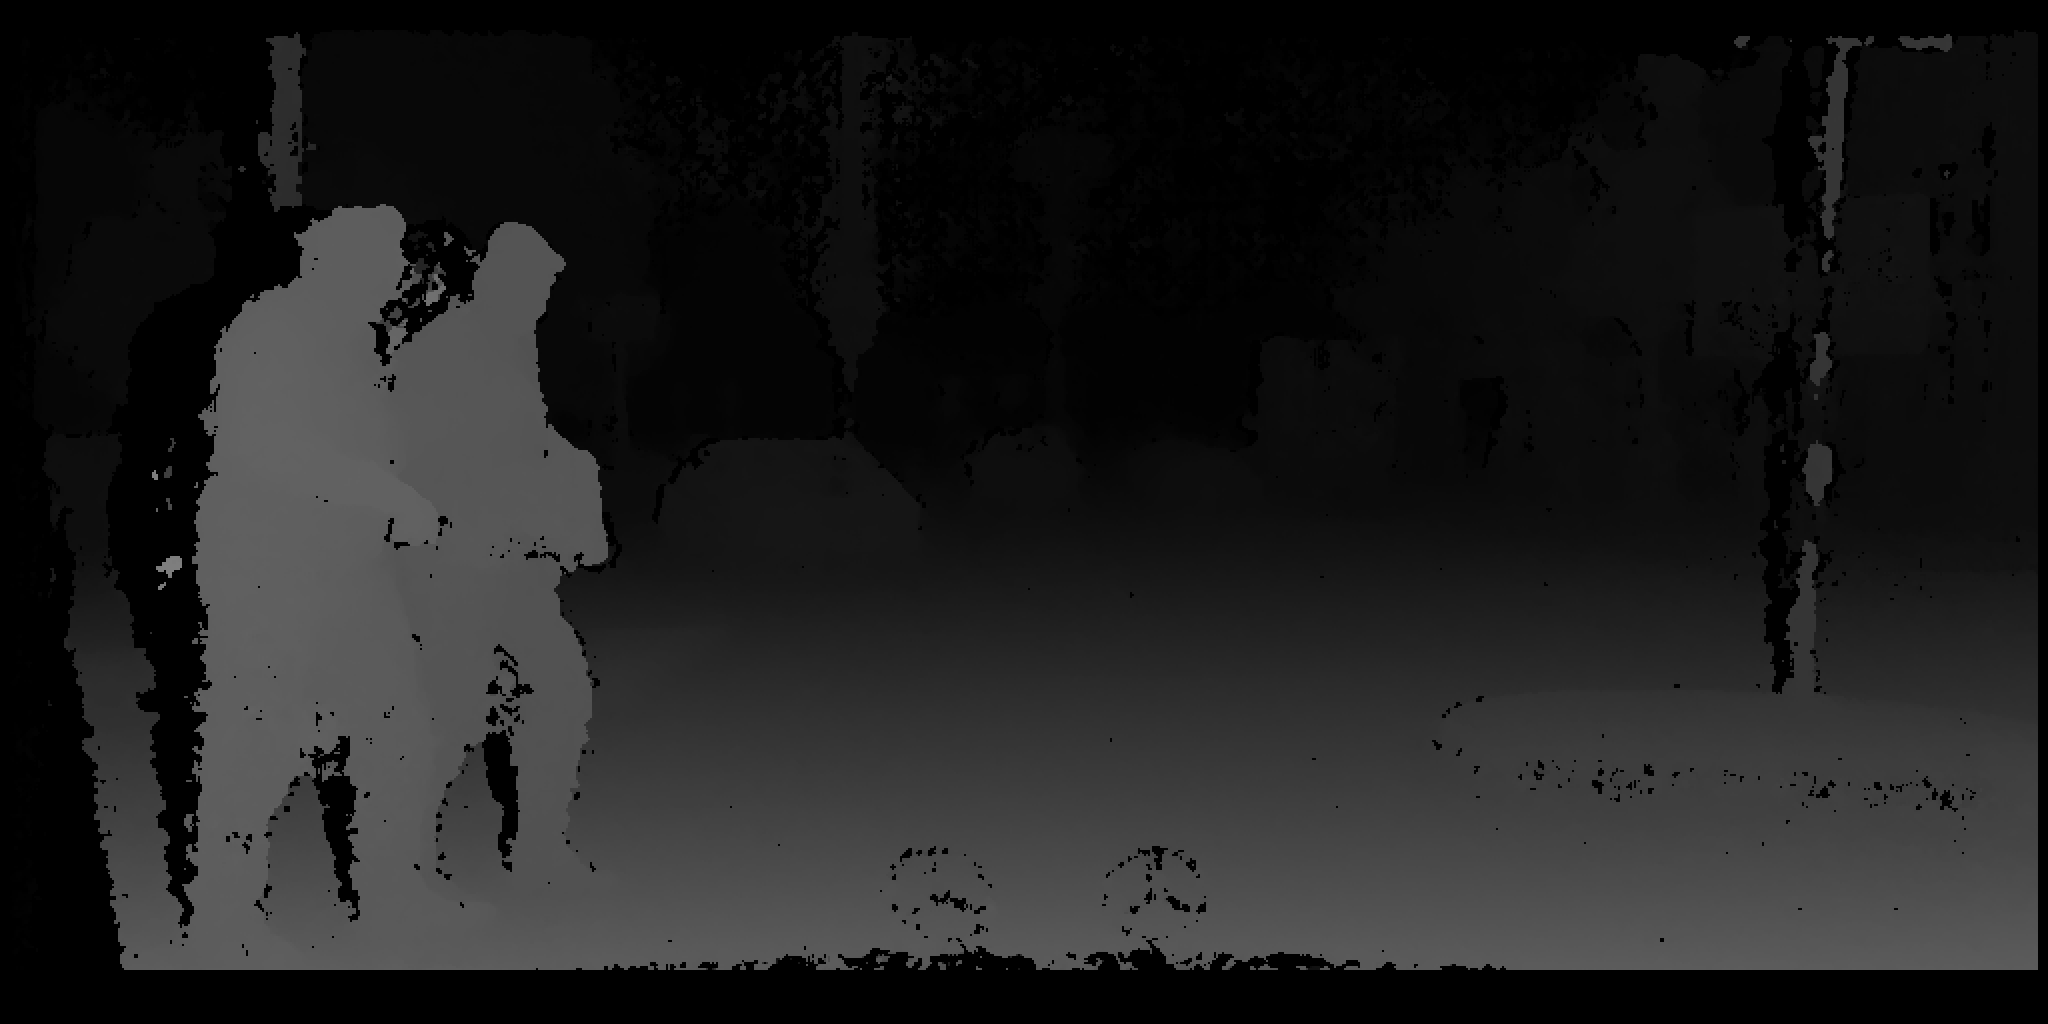
\includegraphics[width=\textwidth]{figures/leverkusen_000024_000019_disparity.png}}{Cityscapes esimerkki kuva leverkusen_000024_000019_disparity}
\caption[Tämä on lyhyt kuvateksti.]{Citysscapes datasetin syvyysdata esimerkki.}
\label{fig:depth}
\end{figure}


\chapter{Aineisto}%
\label{ch:aineisto}

Työn toteuttamiseen käytettiin cityscapes datasettiä \cite{Cordts2016Cityscapes}.


Datasetti pitää sisällään dispariteettidatan, sekä segmentaatiodatan.
Data on autosta stereokameralla kuvattua.
Malli on suunnattu automatisoituun liikenteeseen, ja siinä on paljon erilaisia kaupunkikuvia teiden varsilta.
Tämä tuottaa hankaluuksia lopputuloksen kanssa, sillä malli toimii reaalimaailmassa vain kaupunkikuvissa.
Kuitenkaan yleisempää disparteetti sekä segmentaatiomallia ei järkevästi löytynyt. 
Tämän ongelman olisi voinut kiertää käyttämällä erillisiä malleja segmentointiin sekä dispariteettiin. 
Kahden erialisen mallin yhdistäminen tuo kuitenkin enemmän riskejä.
Kahden mallin tapauksessa, jouduttaisiin joko luottamaan segmentaatiomalliin datan valmistelussa, 
tai kaikki data joduttaisiin käymään manuaalisesti läpi.

Data on kerätty erilaisista kaupunkiympäristöistä, ajoneuvon kyydistä kuvaten.
Tästä johtuen data on melko homogeenistä. Dataan on merkattu monia erilaisia segmentoituja kohteita, niinkuin ihmiisä polkupyöriä ja autoja. 
Tämän työn kannalta kuitenkin tärkeintä on, että kaikki liikkuvat kohteet on merkattu.
Kaikkia kuvia on tarjolla sekä vasemmasta että oikeasta kamerasta kuvattuna.
Data on tämän työn kannalta melko helposti työstettävää. Koska kaikki kuvat ovat ajoneuvosta otettuja, on kuvattava alue rajoittunut alueisiin joissa voi autolla ajaa.
Tämän kuitenkin tuottaa joitain rajoitteita datan käytössä, koska mallin käyttö tämän datasetin ulkopuolisen datan kanssa ei ole kovin helppoa ilman uudelleenkouluttamista.
Kaupungit joista data on kerätty on enimmäkseen sakalaisia kaupunkeja.
Ne ovat kuvatuilla alueilla usein hyvin tiheään rakennettuja. 
Tämä aiheuttaa, että suurella osalla syvyyskartoista on selkeät reunat.

Jotta datasta saataisiin kattavampaa, olisi hyvä keskittyä kuviin jotka on kuvattu muualta kuin kadulta.
Tämän avulla lopullista mallia voisi yleistää toimimaan myös muissa kuin autoteiden tunnistamisessa.
Toinen parantamiskohde dataan voisi olla kuvaaminen kaupunkien ulkopuolelta.
Tälläisiä kuvia ei tästä datasetistä löydy, koska sen pääkäyttökohde on segmentaatio datan käsittelyyn.

\begin{figure}[h]
\centering
\pdftooltip{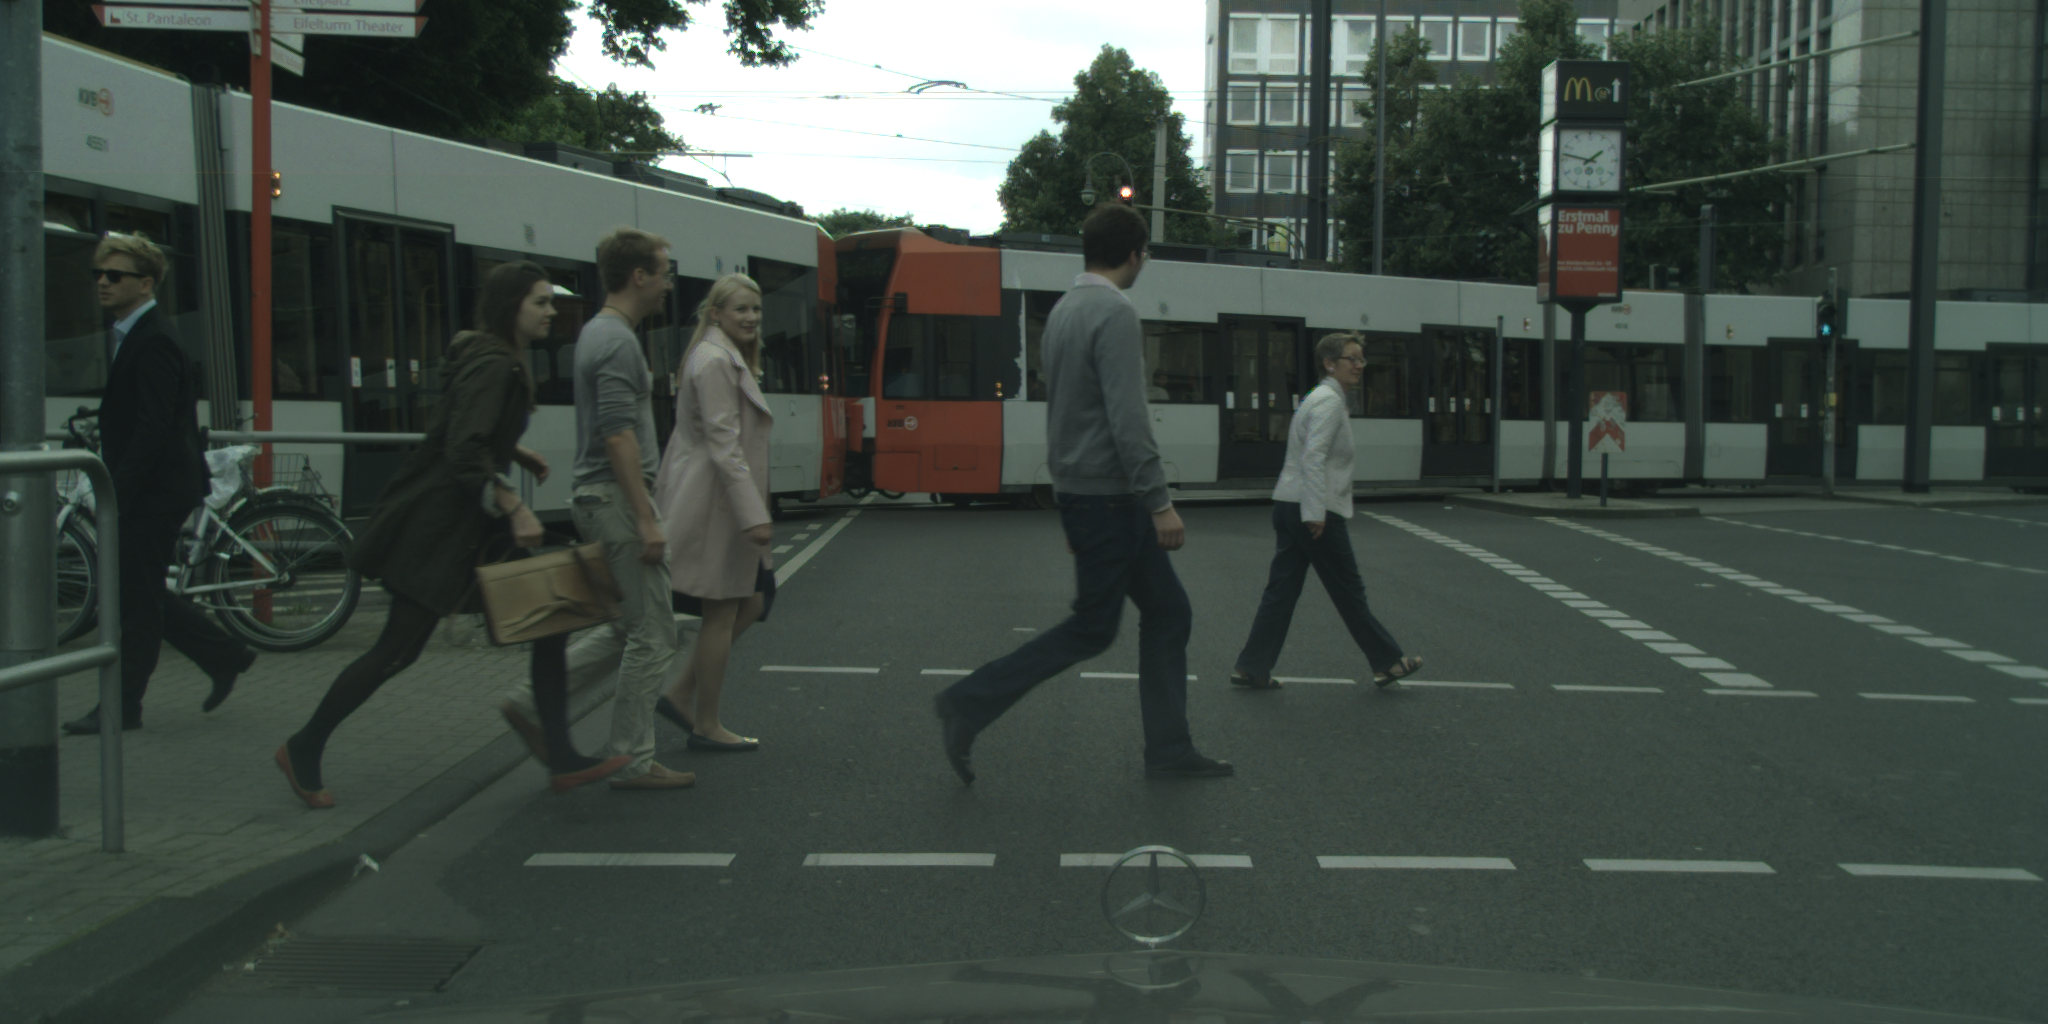
\includegraphics[width=\textwidth]{figures/extreme.png}}{extreme}
\caption{Esimerkki huonosta kuvasta}
\label{fig:extreme}
\end{figure}

    
Aineistossa on myös paljon kuvia jotka ovat "käyttökelvottomia" Kuva \ref{fig:extreme}.
Tämä kuva on hyvä esimerkki tilanteesta jossa edes ihminen ei pysty ilman laajaa taustatietoa arvelemaan mitä liikkuvien kohteiden takana olisi.
Ilman jonkinlaista ulkoista tietoa, tai datan generointia ei vain ole mahdollista tietää mikä haluttu totuus on.
Tämä tietysti on ongelma mitä tässä työssä halutaan ratkaista,
mutta lähtökohtaisesti paras lopputulos saadaan oikealla datalla.
Tälläinen datan generointi ja arvausten tekeminen toki onkin missä neuroverkot ovat omillaan.



\chapter{Metodologia}
\label{ch:metodologia}

Tavoiteltu lopputulos on malli joka palauttaa stereokuvasta syvyysdatan, ilman liikkuvia kohteita.
Manuaalisesti tämän voisi toteuttaa laskemalle kuvista dispariteetti, ja poistamalla tästä dispariteetti kuvasta halutut kohteet.
Jos lähtökohtana on kuvapari, on manuaalinenkin arviointi hyvin likimääräistä. Kuitenkin voidaan ajatella että perusperiaatteeltaan asioiden takana oleva syvyys jatkuu samanlaisena kuin asian ympärillä.
Vaikka tämä ei aina päde, pyritään mallilla testaamaan, onko kappaleen täyttö sitä ympäröivillä syvyyksillä riittävä tekniikka.

\subsection{Stereoanalyysi}

Syvyysdatan ja dispariteetin analysointi tehdään ilman neuroverkkoja.
Tässä tapauksessa se tehdään Hirschmullerin SGM-algoritmillä \cite{hirschmuller2005babel}.
Käytettävä variaatio tästä algoritmistä on OpenCV ssä toteutuettu StereoSGBM \cite{opencvsgbm}.
Seuraava esimerkki Kuva  \ref{fig:disparity1} on luotu function parametreillä, numDisparities=128, blockSize=20, mode=cv2.StereoSGBM\_MODE\_HH
sekä lisäämällä stereo kuviin gaussisen sumennoksen laskennan helpottamiseksi \cite{AnShiyong2021Asvs}.

\begin{figure}[h]
\centering
\pdftooltip{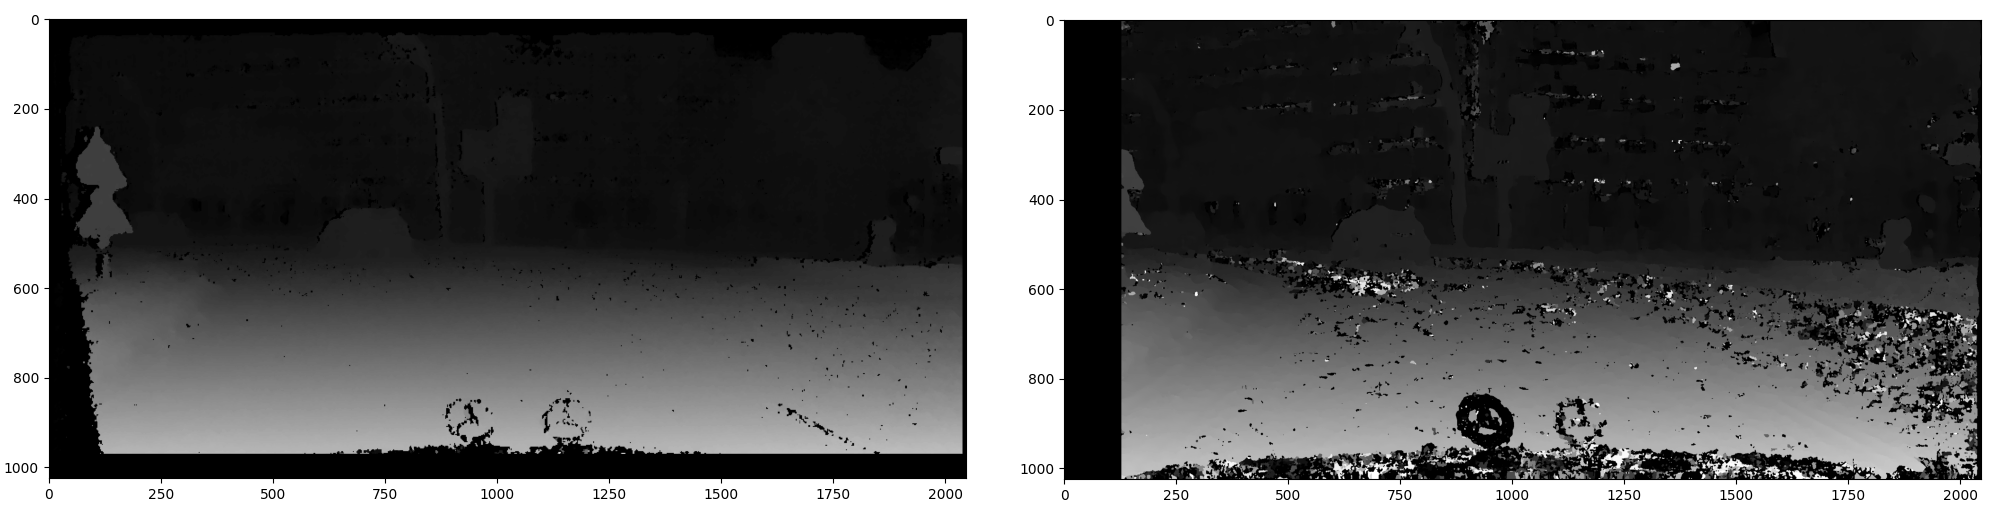
\includegraphics[width=\textwidth]{figures/disparity_1.png}}{disparity example}
\caption[Tämä on lyhyt kuvateksti.]{Vasemmalla tarjottu totuus. Oikealla opencv tulos stereo kuvasta.}
\label{fig:disparity1}
\end{figure}
    
Syvyysdatan kerääminen stereokuvista on mahdollista opencv2 kirjaston avulla.
Sumennus lisättiin jotta mahdolliset kameran aiheuttamat häiriöt saadaan minimoitua.
Käytetyt parametrit tarkoittavat että mahdollisia disparity tasoja on 128 ja alue jolta samankaltaisuutta verrataan on 20 pikselin kokoinen.
Funktiota ajettin HH modessa, joka tarkoittaa että se suoritetaan algoritmin alkuperäisellä suoritustavalla, 
eikä kevennetyllä jota käytetään muistin säästämiseksi.

Tuloksestamme huomaamme häiriötä jota totuudessa ei ole.
Tämä johtuu todennäköisesti kohdista kuvista joista Hirschmullerin-algoritmi ei pysty tunnistamaan vastaavaa kohtaa toisessa kuvassa.
Tämä voi tapahtua esimerkiksi asfaltin pinnassa jossa on hyvin samankaltaista tai varjoisilla alueilla. 

Tässä tilanteessa voisimme myös kouluttaa verkon jonka avulla saisimme hankittua syvyysdata,
mutta koska syvyysdata ei ole yleisesti saatavilla olevaa koulutusdataa,
ei voida olettaa että se olisi saatavilla tulevissa toteutuksissa. 

\subsection{Semanttinen Segmentointi}

Aineistossa on jo olemassa totuus segmentaatiodatasta.
Käytämme tätä valmista dataa, mutta koulutamme silti sitä varten myös uuden verkon.
Koulutettu verkko on hyvin yksinkertainen ja käyttää valmiita pytorch komponentteja.
Data on koulutettu\ fcn\_resnet50 avulla \cite{pytorchfcnresnet50}, ilman esikoulutettuja painoja. Optimointiin on käytetty Adam-algoritmia ja häviöfunktioksi on valittu CrossEntropyLoss-funktio.
Datasetin mallia on yksinkertaistettu tarpeen mukaan: kaikki liikkuvat kohteet, kuten autot ja ihmiset, on yhdistetty yhdeksi luokaksi ja kaikki muu toiseksi luokaksi.
Näin saadaan yksinkertaisempi malli, jonka avulla voidaan kuvasta tunnistaa kaikki liikkuvat kohteet Kuva \ref{fig:segmentation1}.

\begin{figure}[h]
\centering
\pdftooltip{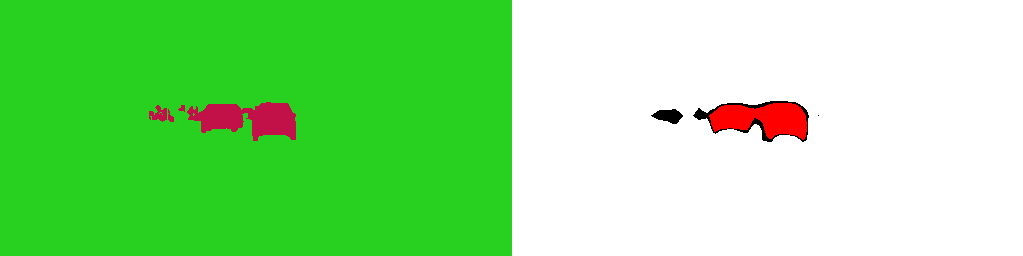
\includegraphics[width=\textwidth]{figures/segmentation1.png}}{segmentation example}
\caption[Tämä on lyhyt kuvateksti.]{Vasemmalla tarjottu totuus. Oikealla mallin tuottama.}
\label{fig:segmentation1}
\end{figure}
    

Tällä tavalla tehty malli antaa meille riittäviä tuloksia alkuperäiseen totuuteen verrattuna.
Ja sen kouluttaminen on myös melko yksinkertaista.
Tätä mallia ei kuitenkaan tarvita kuin lopullisen mallin luomiseen mahdollisissa muissa käyttökohteissa, joissa dataa ei ole saatavilla.
Voi kuitenkin olla helpompaa segmentoinnin sijaan, arvioida suoraan asioiden alla oleva syvyys.
Kuitenkin jos data tuotetaan esimerkiksi useilla kuvilla samoista kohdista joissa kohteet liikkuvat,
on segmentaatio mallista enemmän hyötyä.
Koska sitä voisi tälläisissä tapauksissa käyttää pelkästään taustasyvyys arvioinnin tuottamiseen, ilman syvyyksien arvaamista.

\section{Datan muodostus}

Niin kuin aikaisemmin jo mainittu, tavoite on jalostaa data muotoon, jossa kaikki liikkuvat kohteet on hävitetty syvyysdatasta.
Koska käytetty data on kaupunkidataa, tämä tarkoittaa autojen sekä ihmisten poistamista kuvista.
Koska käytettävissämme on kuvien segmentaatiodata, voidaan niiden alue poistamalla dispariteetista saavuttaa tila, jossa niitä ei oteta huomioon.

Kun liikkuvien objektien alue on poistettu, pitää niiden alla oleva alue generoida jotenkin. 
Kyseisten alueiden alla voi olla miltei mitä tahansa, 
ja ei ole selkeää ja helppoa keinoa sitä tietää. 
Alueen alle voi jäädä taloja joissa on erikoisia kulmia, puita, pensaita postilaatikoita tolppia ja mitä tahansa muuta. 
Tästä johtuen ei voida olettaa, että kyseinen malli olisi erityisen tarkka.
Kuitenkin alueen karkeaan arviointiin tuotetun datasetin pitäisi olla riittävä.
On tärkeä muistaa, että huonosti toteutettu dataset tuottaa myös huonoja tuloksia tuottavan mallin.

Tässä työssä mallin käsittelyä yritettiin vertikaalisella ja horisontaalisella pyyhkäisyllä, sekä niiden yhteistuloksella.
Tämä tarkoittaa että jokainen yhtenäinen alue etsittiin ja niiden syvyysarvot otettiin niiden reunoilta,
ja pyyhkäistiin läpi täsmäämään vastakkaisen reunan arvoon.
Tämä tarkoittaa, että jos kohteen takana on esimerkiksi puu vertikaalinen pyyhkäisy osaisi ottaa sen huomioon.
Jos kohteen takana sen sijaan on aita vertikaalien pyyhkäisy osaisi ottaa sen huomioon.
Ja yhdistetyssä tavassa nämä arvot on summattu, joten sen pitäisi olla keskiarvoltaan hyvä. 

\begin{figure}[h]
\centering
\pdftooltip{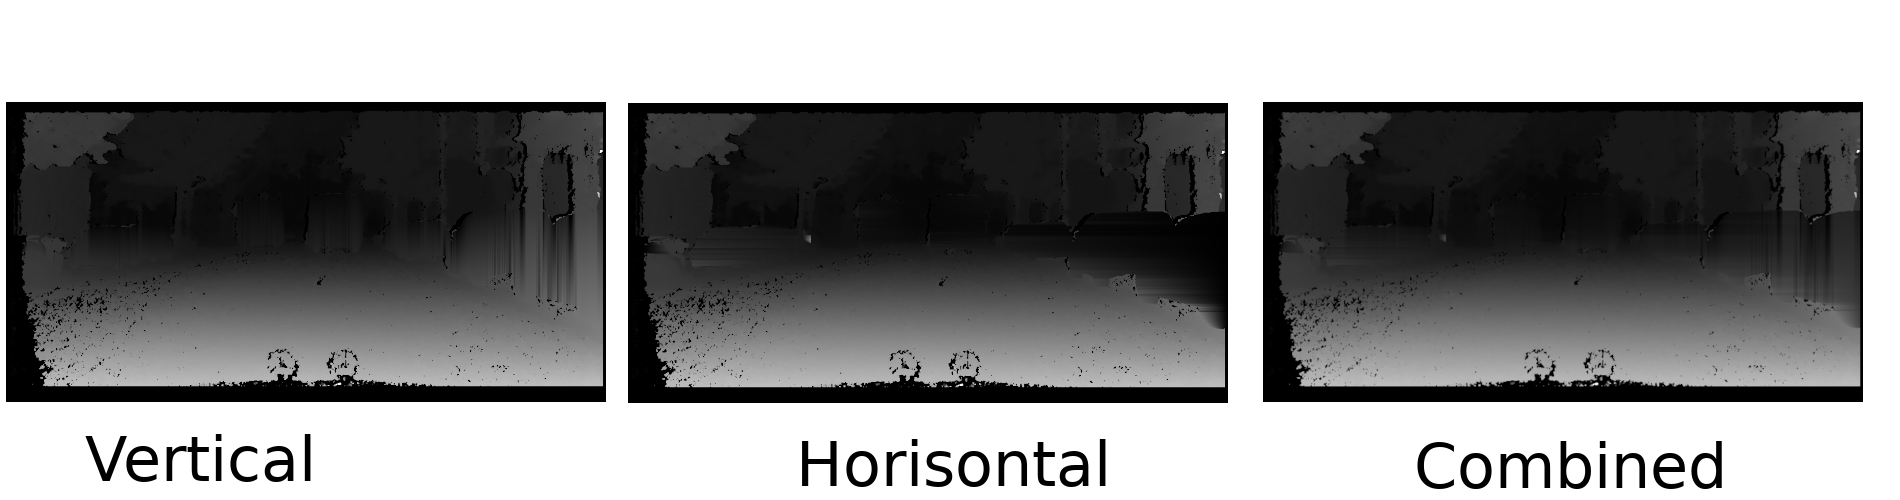
\includegraphics[width=\textwidth]{figures/swipe.png}}{Swipe}
\caption{Eri tyypin pyyhkäisyt syvyyden arviointiin}
\label{fig:swipe}
\end{figure}


Tässä kuvassa Kuva \ref{fig:swipe} on esitelty tavat vertikaali horisontaali sekä niiden yhdistetty arvo. 
Siitä huomataan että mikään tavoista ei ole täydellinen.
Tästä johtuen jotta datasta saadaan edes jollain tavalla käytettävää, tulee se käydä ensin läpi. 

Kuvien manuaalisessa valinnassa vertailtiin yllä mainittujen kuvien lisäksi pyyhkäisyjä,
jotka ylittävät tunnistetun reunan 50:llä pikselillä.
Datan läpikäynnin jälkeen valituksi tuli seuraavanlaisia kuvia.

\begin{figure}[h]
\centering
\pdftooltip{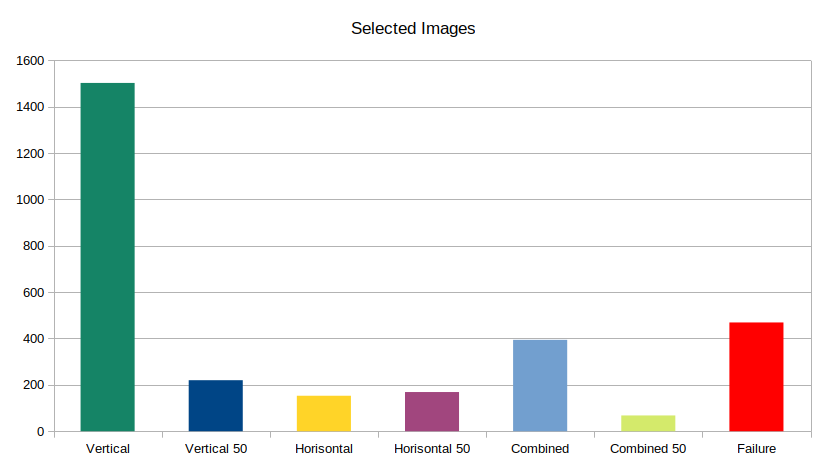
\includegraphics[width=\textwidth]{figures/selectedimages.png}}{Selected}
\caption{Valitut kuvat}
\label{fig:selected}
\end{figure}

Tästä huomaamme että vertikaalinen valinta oli yleisin Kuva \ref{fig:selected} .
Yleensä jos horisontaalista dataa tarvittiin, se yleensä kannatti yhdistää vertikaalidataan.
Tämä johtuu todennäköisesti datan luonteesta. Suuri osa kohteista on melko lähellä kameraa ja reunassa.
Tämä johtaa tilanteeseen jossa analysoitavan alueen oikealla tai vasemmalla puolella ei ole tarpeeksi syvyysdataa jota voisi käyttää syvyyden generoimiseen.
Vertikaalipyyhkäistyjen kuvien data on myös todennäköisemmin oikein, koska suurin osa datasta on tieltä joka jatkuu eteenpäin.
Näin ollen ylempänä kuvassa kauempana oleva tasainen pyyhkäisy on todennäköisemmin oikein, kuin vasemmalta oikealle tuleva, joka tuo tulokseen enemmän satunnaisuutta.
Näin ollen koska kuvat on käsin silmämääräisesti valittuja, luonnollisimman näköiset kuvat ovat todennäköisesti valittuja.
Yhden kuvan valitsemiseen ei kuitenkaan ole käytetty paljoa aikaa vaan se on hyvin ”fiilis pohjaista”.

Yleisimmät asiat mitkä toivat ongelmia, olivat segmentoitujen alueiden vieressä olevat epäselvyydet.
Sekä alueet jotka olivat niin reunassa että niiden vierest käytettävän syvyyden saanti ei ollut mahdollista.
Jatkokehityksessä näitä ongelmia voisi yrittää parantaa muutamilla tavoilla. 

Tunnistettuja alueita laajentamalla voisimme onnistua piilottamaan joitan tunnistettujen alueiden reunoilla esiintyviä syvyysdatan häiriöitä.
Koska emme ole kiinnostuneita tunnistamaan asioita vaan piilottamaan ne, ei kovin suuri tarkkuus ole tarpeellista.
Jälkianalysoinnin kannalta myöskin liian suuri alue on huomattavasti pienempi harmi kuin liian pieni alue.

Tulosta voisi myös parantaa siistimällä disparitaatiodatasta kohinaa suodattamalla.
Tämä todennäköisesti poistaisi jotain tärkeää dataa,
mutta jälleen kerran tavoiteltu tarkkuus ei ole niin suuri että tästä pitäisi koitua suuresti haittaa,
koska yleinen ongelma on, että dataa ei ole saatavilla kuvan ulkopuolelta.

Koulutsdatan kuville voitaisiin luoda syvyyttä arvioiva kehys.
Tämä varmistaisi että syvyys on aina saatavilla, 
ja tällaisen kehyksen generointi pitäisi olla mahdollista datan samankaltaisuudesta johtuen.

Yksi yleisesti ongelmia tuottava tunnistettu kohde ovat ihmiset.
Ihmiset ovat monimutkaisempia muotoja kuin autot.
Näin ollen myös mallissa, ihmisen erottelu on tarkempaa.
Kuitenkin joissain kuvissa,
jos ihminen peitetään pienimmän ja suurimman koordinaatin peittävällä kuutiolla,
menetetään paljon dataa jota, ihmisen ympäriltä on havaittavissa.
Tätä varten voisi olla hyöydyllistä kirjoittaa algoritmi joka arvioisi muutoksen alueella olevia suurimpia eroja,
ja ehkä suodattaa suurimmat muutokset pois. Näin menetettäisiin osa datasta,
mutta todennäköisesti myös suurimmat virheet saataisiin hävitettyä. 

Tällä tavalla tuotettu malli, vaatii paljon manuaalista työtä ja hyväksyntää.
Kuitenkin kun uusia malleja tehdään, ei niiden luomiseen ole oikoteitä.
Kuitenkin mitä enemmän tätä työtä tehdään,
sitä helpommaksi se olemassa olevan mallin avulla tulee.
Manuaalisesta työstä ei kuitenkaan koskaan pääse datan validoinnissa pois,
jos käytössä ei ole parempaa lähtödataa.
Jos datasetti muodostettaisiin ottamalla samasta kohdasta useita kuvia,
niin kauan että kaikki liikkuvat kohteet olisivat poistuneet,
voitaisiin sen ja segmentaatiomallin avulla luoda huomattavasti parempaa koulutusdataa. 

\section{Ensimmäinen malli}

Datasta koulutettiin malli samalla pytorchin tarjoamalla "fcn\_resnet50" \cite{pytorchfcnresnet50} neuroverkolla kuin segmentaatiovaiheessa.
Ulostulon muoto jaettiin 128 luokkaan, jotka vastaavat eri syvyyttä.
Sisääntulona annettiin 2 harmaata kuvaa 3-ulotteisen matriisin eri kerroksissa.
Näin voitiin käyttää valmista segmentaatio mallia värikuva sisääntulolla, kahden stereo-mustavalkokuvan analysointiin ja tuottaa sillä syvyyskartta.

\begin{figure}[h]
\centering
\pdftooltip{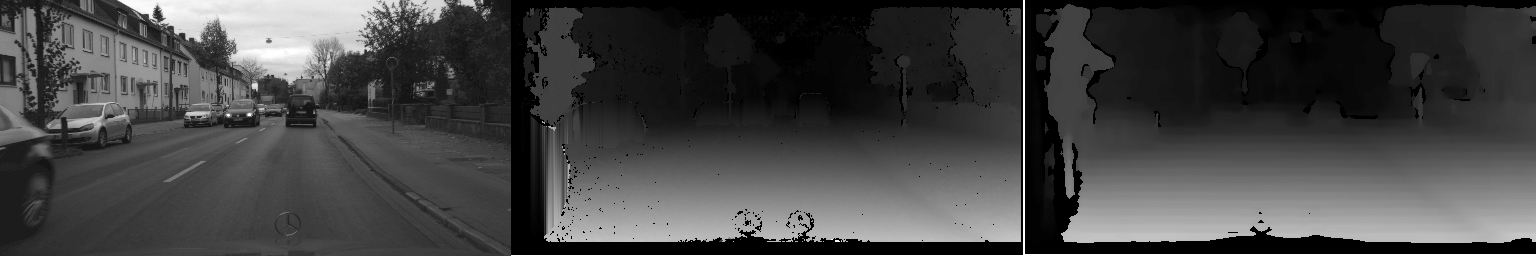
\includegraphics[width=\textwidth]{figures/model.png}}{Model}
\caption{Kuvassa vasemmalta oikealle; alkuperäinen kuva, rakennettu totuus, koulutetun mallin lopputulos.}
\label{fig:model}
\end{figure}



Kuvasta Kuva \ref{fig:model}  nähdään että, koulutus itsessään pystyy tuottamaan hyvin samankaltaisia kuvia kuin laskettu malli. Koulutettu malli kuitenkin oletetusti perii koulutusdatan heikkoudet. Koska käytetty automatisoitu tapa ei tuota täydellistä dataa, ei myöskään koulutettu malli ole täydellinen. 


\section{Datan jatkojalostus}

Jotta mallista saataisiin parempi täytyy koulutusdataa pyrkiä jalostamaan tehokkaammin. 
Aikaisemmat prosessointi tavat olivat melko yleisiä ja käytettäviä millä tahansa datalla. Paremman lopputuloksen saamiseksi voi olla tarpeellista on erikoistuneempia datankäsittelytapoja.
Käytetty koulutusdata on kaupunkidataa. Tästä johtuen se on hyvin homogeenistä.
Voimme käyttää tätä hyväksemme kun yritämme arvioida kohteiden takana olevaa syvyyttä.

\begin{figure}[h]
\centering
\pdftooltip{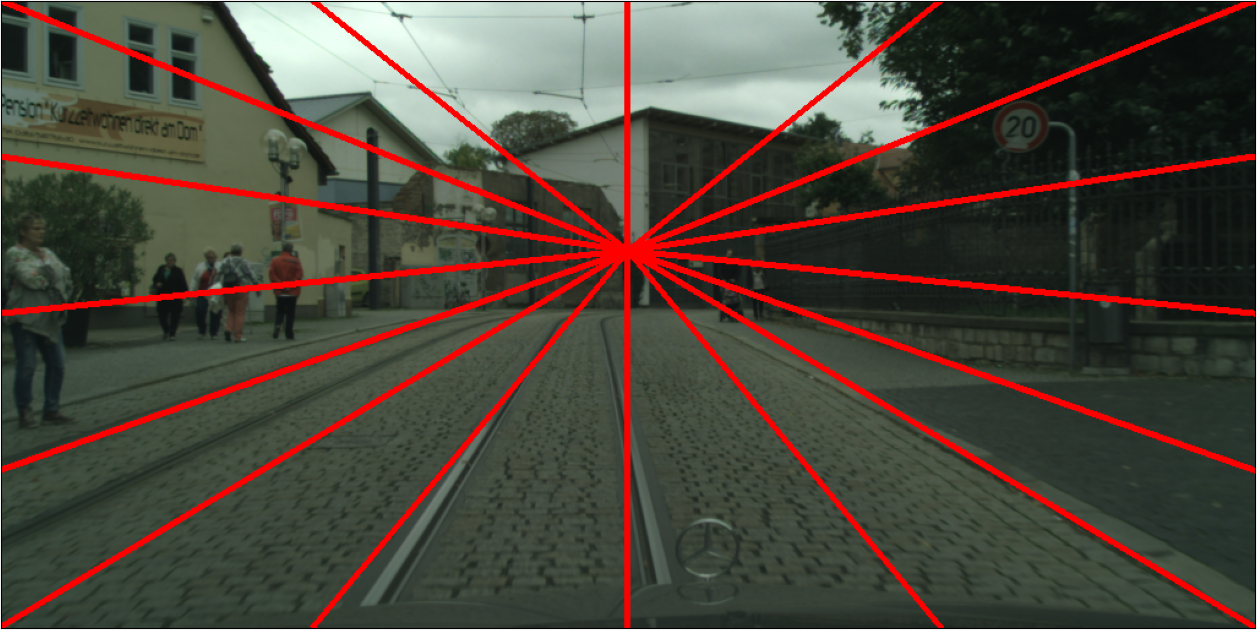
\includegraphics[width=\textwidth]{figures/focal_image.png}}{Model}
\caption{Kuvassa Esimerkki "polttopisteestä"}
\label{fig:polttopiste}
\end{figure}


Kaupunkiympäristössä kuva on usein otettu samankaltaisesta asetelmasta tiellä ajavasta autosta. 
Tästä johtuen voimme arvioida syvyyden muutoksen tapahtuvan hyvin samankaltaisesti eri kuvausajankohtina.
Tämän arvion voimme tehdä arvioimalla "polttpoisteen" jossa todennäköisesti on kuvan suurin syvyys Kuva \ref{fig:model},
poislukien taivas eli ainakin kuvan merkitsevän alaosan osalta. Vaikka esimerkkikuvassammekaan syvyys ei asetu täysin arvioituun kohtaan.
On se silti tarpeeksi lähellä jotta sitä voitaisiin käyttää. 
Kun yhdistämme tähän geneerisissä tavoissa käyttämämme pyyhkäysy tekniikan jonka suoritamme polttopisteen suuntaan.
Saamme aikaan syvyyden muutoksen joka on luonnollisemman oloinen todelliseen syvyysdataan nähden.

Tämän lisäksi voimme lisätä arvion syvyydestä kuvan eri alueilla. 
Tämä helpottaa syvyyden arvioita tilanteissa joissa korvattava kohde alkaa jo kuvan reunalta.

\begin{figure}[h]
\centering
\pdftooltip{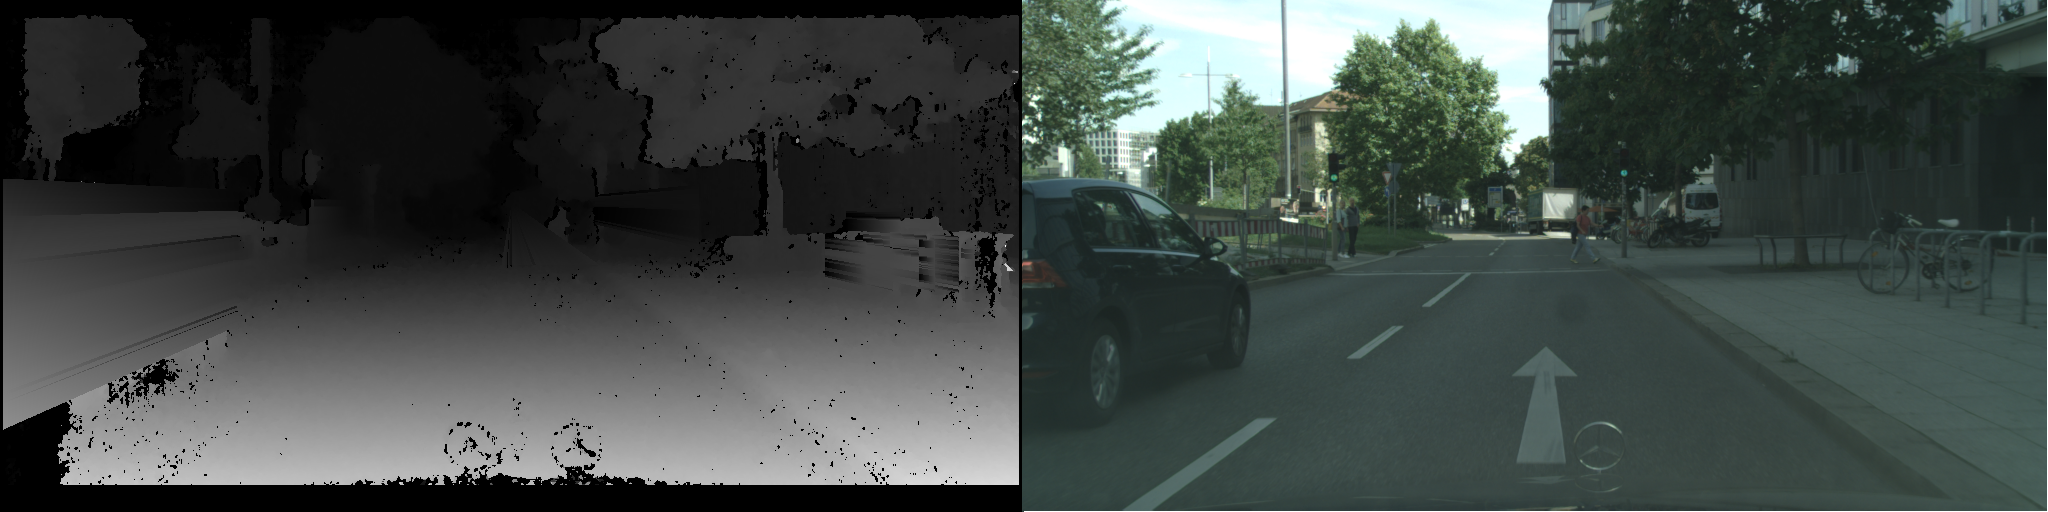
\includegraphics[width=\textwidth]{figures/focal_depth.png}}{Model}
\caption{Esimerkki syvyyden arvioinnista polttopistettä kohti}
\label{fig:polttopiste_2}
\end{figure}
    
Kuvassa \ref{fig:model}, näemmä että vasemmassa reunassa oleva auto alkaa suoraan kuvan reunalta.
Näin ollen emme voi kuvasta tarkistaa alkavaa syvyyttä ennen autoa.
Tässä voimme käyttää likimääräsistä arvoita syvyyksistä kuvan eri alueille. Vaikka saamanne lopputulos ei ole täydellinen,
on se silti toimiva lähtökohta syvyyden korvaamiselle.

Koska kyseessä on pelkästään käyttämäämme dataa varten valittu tekniikka, ei se tuota hyviä tuloksia kuin sen kanssa yhteensopivaan dataan.
Vaikka suuri osa data onkin keskenään samankaltaista. Ei kuitenkaan kaikkien kuvien prosessointi ole järkevää sen avulla.
Manuaalisen läpikäynnin jälkeen huomaamme, että kuitenkin vain noin neljäsosa kuvista on tuottanut parhaan prosessointi lopputuloksen focal eli polttopiste tekniikan avulla. 

\begin{figure}[h]
\centering
\pdftooltip{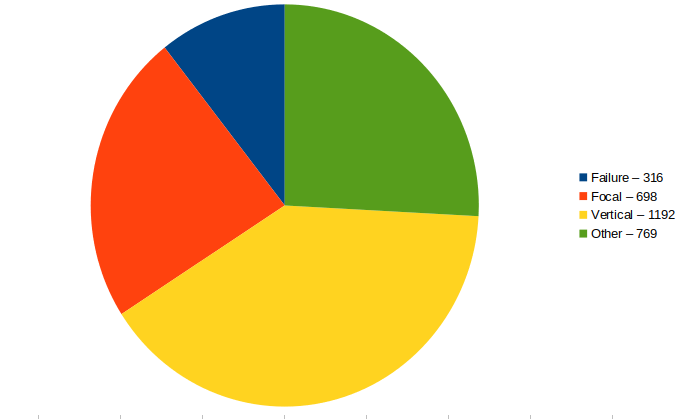
\includegraphics[width=\textwidth]{figures/NewChart.png}}{Selected2}
\caption{Uudet Valitut kuvat}
\label{fig:selected2}
\end{figure}

Uusi tapa on kuitenkin ratkaissut osan kuvista joiden reuna alueet ovat olleet täynnä autoja. Siirtäen ne epäonnistuneiden kuvein osastolta testaukseen käytettäviin kuviin.

\section{Lopullinen malli}

Lopullinen tuotettu malli, on tehty samalla tavalla kuin ensimmäinenkin.
Sen kouluttamiseen on vain käytetty hieman erilaista dataa. Sen toiminnan paremmuuden tietellinen analysointi ei anna kuitenkaan realistisia lopputuloksia.
Alkuperäinen data sisältää niin paljon häiriötä ja epäpuhtauksia, että sen arvioinnin tarkkuus on hyvin hankalaa.

\begin{figure}[h]
\centering
\pdftooltip{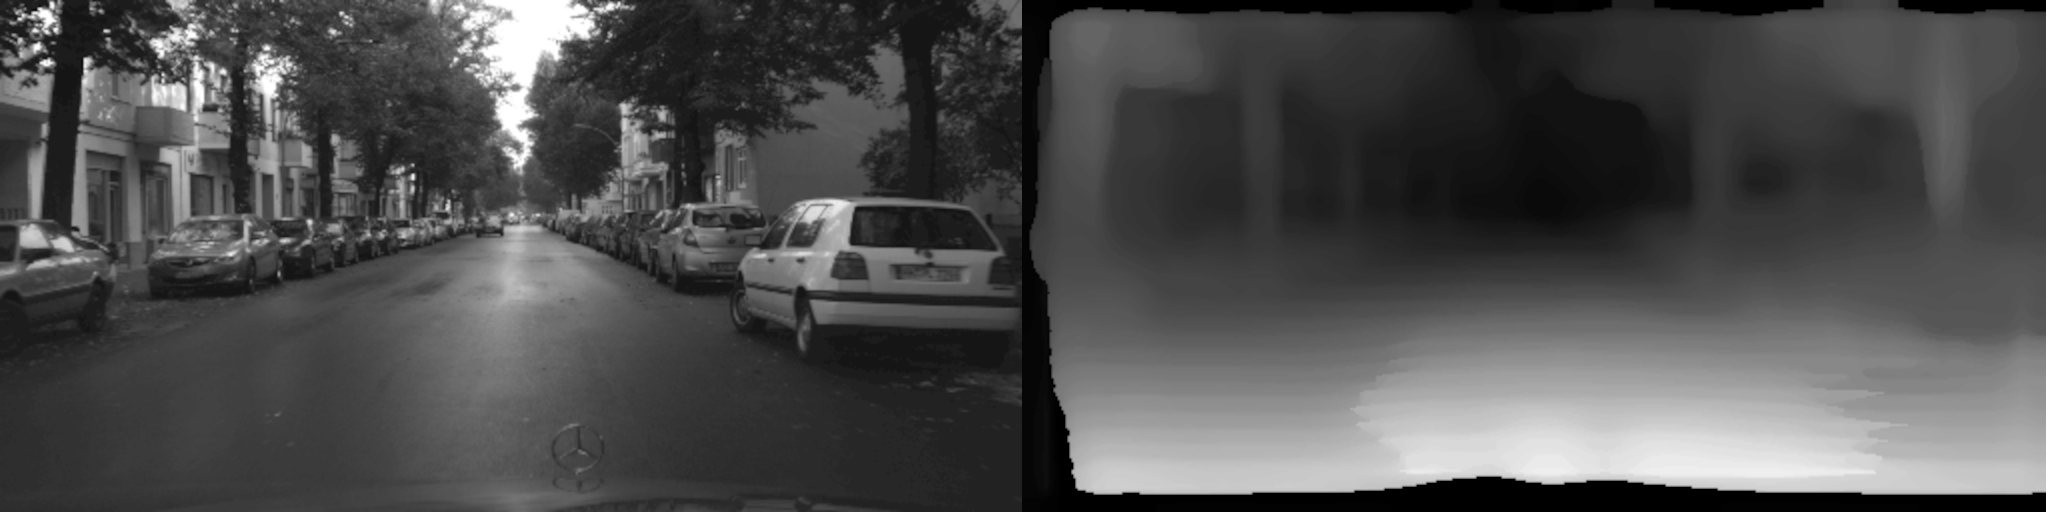
\includegraphics[width=\textwidth]{figures/new_model.png}}{uusi_malli}
\caption{Uuden mallin lopputulos}
\label{fig:uusi_malli}
\end{figure}


Vaikka malli saavuttaisikin "täydellisen" lopputuloksen ei se silti tuota haluttuja tuloksia, koska koulutusdata ei ole täydellistä.
Tuotettu lopullinen malli onkin mielestäni tästä johtuen hyvä, vaikka sen tuottama kuva onkin "sumea". 
Tämä sumeus auttaa piilottamaan epätarkkuuksia, ja todennäköisesti olisi riittävä mahdollisissa reaalimaailman käyttökohteissa.
Kuvassa Kuva \ref{fig:uusi_malli} nähdään että uusi malli pystyy arvioimaan syvyyden autotien sivussa olevien autojen takaa. 
Se myös pystyy joissain määrin arvioimaan autojen takana olevian puiden runkojen syvyyden. 
Se on myöskin piilottanut autot silmämääräisesti paremmin kuin vanhassa kuvassa, jossa autojen ääriviivat olivat havaittavissa himmeästi.


% \chapter{Esitystyyli}%
\label{ch:esitystyyli}

Tekstin sisällön lisäksi esitystyyli vaikuttaa suuresti viestinnän onnistumiseen. Ulkoasu ja kirjoitustyyli antavat työstä ja kirjoittajasta kuvan, toivottavasti hyvän.

\section{Teksti}

Älä suotta murehdi tekstin asettelusta, tämä pohja hoitaa sen jo valmiiksi. Kirjoitustyylin perusohjeet ovat:

\begin{itemize}
\item Ajattele lukijaa aina tekstiä kirjoittaessasi ja johdattele häntä riittävästi. Anna ensin yleiskuva ja liitä siihen yksityiskohdat.
\item Korosta tärkeimmät asiat, esimerkiksi nostamalla ne omiksi luvuikseen (\verbcommand{section}, \verbcommand{subsection}), poimimalla taulukkoon tai selittämällä kuvan avulla. Tekstissä käytä korostamiseen kursivointia (\verbcommand{emph}), mutta älä korosta liikaa.
\item Vältä pitkiä virkkeitä ja monimutkaisia lauserakenteita. Piste on paras välimerkki.
\item Suosi aktiivimuodossa olevia verbejä ja sijoita ne lauseen alkupuolelle. Älä kuitenkaan käytä yksikön 1. persoonaa (minä) kuin alkusanoissa.
\item Vältä kapulakielisiä ilmauksia ja ammattislangia. Sano asiat suoraan. Käytä vakiintunutta teknistä sanastoa, merkintöjä ja neutraalia asiatyyliä.
\item Lukujen ja alalukujen tulee olla vähintään kahden kappaleen mittaisia ja mielellään keskenään tasapainoisia. Kappale muodostuu aina useammasta kuin yhdestä virkkeestä.
\item Luvut ja alaluvut numeroidaan korkeintaan kolmannelle tasolle (\verbcommand{subsection}) asti, esimerkiksi 4.4.2. Pohja huolehtii tästäkin automaattisesti.
\item Lyhenteitä ei tulisi käyttää liikaa. Käytä lyhenteissä pieniä ja isoja kirjaimia johdonmukaisesti.
\end{itemize}

\section{Lauseympäristöt}

Tiedostossa \code{preamble.tex} on määritelty lauseympäristöjä matemaattisen
tekstin kirjoittamista varten. Näistä esimerkkeinä toimivat suomen- ja
englanninkieliset lauseet~\ref{lause:pythagoras} ja \ref{theorem:pythagoras}.

\begin{lause}[Pythagoraan lause]\label{lause:pythagoras}
    Suorakulmaisen kolmion sivujen \(a\), \(b\) ja \(c\) pituuksille on voimassa yhtälö
    \begin{equation}\label{yht:pythagoras}
        a^2 + b^2 = c^2\,,
    \end{equation}
    jos \(c\) on hypotenuusa.
\end{lause}

\begin{theorem}[Pythagorean theorem]\label{theorem:pythagoras}
    For the sides of a right triangle, \(a\), \(b\) and \(c\), the equation
    \begin{equation}\label{eq:pythagoras}
        a^2 + b^2 = c^2
    \end{equation}
    holds, if \(c\) is the hypotenuse.
\end{theorem}

Tällä hetkellä määritellyt ympäristöt ovat \code{maaritelma}, \code{lause},
\code{apulause}, \code{seurauslause} ja \code{esimerkki}, sekä vastaavat
englanninkieliset ympäristöt \code{definition}, \code{theorem}, \code{lemma},
\code{corollary} ja \code{example}. Näitä on suotavaa käyttää silloin, kun
tekstissä esitellään jokin tärkeä tulos tai määritelmä, johon tarvitsee
viitata myöhemmin. Liika lauseympäristöjen käyttö johtaa kuitenkin
listamaiseen Landaun kirjoitustyyliin, joka ei ole kovin helppolukuista, ja on
sopivaa vain referenssityylisissä teksteissä, joista vain haetaan faktoja.
Diplomityö ei ole tällainen tekstityyppi.


\section{Kuvat}

Kaikkiin kuviin täytyy viitata tekstissä. Kuvan avulla voidaan esittää tietoa tiiviissä muodossa, mutta kuvan täytyy olla merkityksellinen työn sisällön kannalta ja kuva täytyy selittää tekstissä. Viittaus on mielellään samalla sivulla kuin kuva tai sitä ennen. Kuvat ja taulukot numeroidaan ja sijoitetaan pääsääntöisesti sivun yläreunaan, oman harkinnan mukaan. \LaTeX{}issa tämä tapahtuu sijoittamalla \verbcommand{caption}-komentoa seuraavalle riville \verbcommand{label}-komennon, jonka argumentti on kyseisen kuvan (tai taulukon) yksikäsitteinen tunniste. Viittaaminen tapahtuu \verbcommand{ref}-komennolla, johon syötetään haluttu tunniste. Lukua ei saa aloittaa (eikä mielellään lopettaa) kuvalla, taulukolla, kaavalla tai luettelolla, vaan sen ympärillä on oltava tekstiä. Kuvateksti sijoitetaan kuvan alle.

Kuvan keskeinen sisältö on selitettävä tekstissä, jotta sen sanomasta ei jää epäselvyyttä. Analysointiohjelmistojen tuottamat kuvat vaativat useimmiten muokkausta, kuten kuvassa \ref{fig:huolittelu}. Kuvan tekstien on oltava luettavissa, ja niiden kooksi suositellaan samaa kuin muussa tekstissä, 11 pt. Pyri siihen, että myös harmaasävyissä tulostettu kopio on luettava ja selkeä. Suosi vektorimuotoisia kuvatiedostotyyppejä \texttt{.eps} ja \texttt{.pdf} (\LaTeX{} ei syö \texttt{.svg}-tiedostoja\ldots), sillä niitä voi skaalata helposti laadun heikkenemättä. \LaTeX{} sisältää myös erittäin ilmaisuvoimaisia paketteja vektorigrafiikan (\texttt{tikz}) \parencite{tikz} ja kuvaajien (\texttt{pgfplots}) \parencite{pgfplots} piirtämiseen. Kuvassa \ref{fig:pgf-esimerkki} esitetään esimerkki jälkimmäisen avulla luodusta kuvaajasta.

\begin{figure}
\centering
%\begin{subfigure}{0.49\textwidth}
\pdftooltip{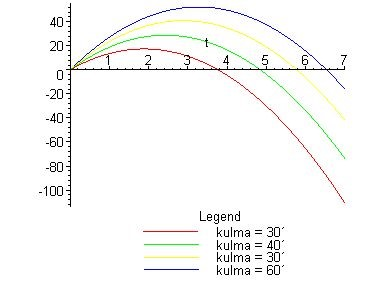
\includegraphics[width=\textwidth]{figures/bad-example.jpg}}{Kuva. Neljä alaspäin aukeavaa kaarta alkaa origosta eri lähtökulmilla. Kuvaajan skaalaus on huono ja akseleita ei ole nimetty johdonmukaisesti.}
%\end{subfigure}
%\begin{subfigure}{0.49\textwidth}
\pdftooltip{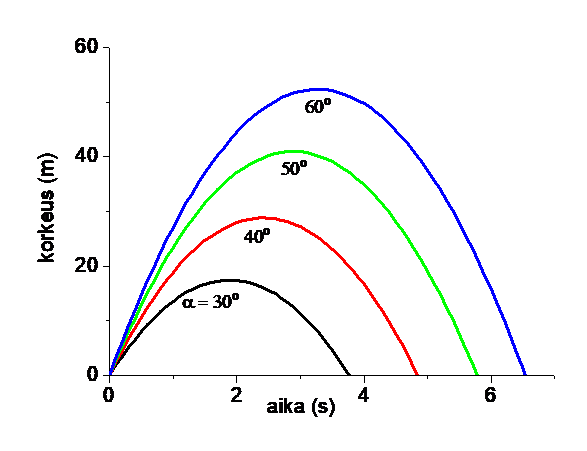
\includegraphics[width=\textwidth]{figures/good-example.png}}{Kuva. Neljä alaspäin aukeavaa kaarta alkaa origosta eri lähtökulmilla. Kuvaaja on skaalattu selkeäksi, akseleilla on täsmälliset nimet ja jokaiseen kuvaajaan liittyvä lähtökulmatieto on merkitty sen viereen.}
%\end{subfigure}
\caption[Tämä on lyhyt kuvateksti.]{Kuvaaja on hyvä muokata julkaisukelpoiseksi. Vasemmalla on esitetty muokkaamaton kuvaaja ja oikealla muokattu.}
\label{fig:huolittelu}
\end{figure}

\begin{figure}
\centering
%\input{figures/pgf-example.tex}
\caption{Kuvan \ref{fig:huolittelu} tyylinen esimerkki \texttt{pgfplots}-paketilla piirrettynä.}
\label{fig:pgf-esimerkki}
\end{figure}

\section{Taulukot}

Taulukot sopivat hyvin erityisesti numeerisen informaation esittämiseen tiiviissä muodossa. Kuvien tapaan taulukot numeroidaan ja varustetaan otsikolla, kuten taulukossa. Taulukkoteksti sijoitetaan samalle sivulle taulukon kanssa ja taulukon yläpuolelle. Suureet, lyhenteet ja symbolit selitetään tarvittaessa tekstissä. Kaikkiin taulukoihin on viitattava tekstissä, mieluummin ennen taulukkoa. Taulukon keskeinen sanoma ja tulkintaohjeet selitetään tekstissä.

Taulukon sarakkeet otsikoidaan, ja suureet sekä yksiköt laitetaan näkyviin. Jos otsikkoriviä tarvitsee erottaa muusta taulukosta, tee se korostamalla (\verbcommand{emph}). Taulukon järjestyksellä on suuri merkitys. Jokaista solua ei pidä ympäröidä reunaviivalla, koska taulukosta tulee raskaslukuinen. Lisää vaakaviiva taulukon ylä- ja alareunaan. Vaakaviivoja voi käyttää esimerkiksi 4--5 rivin välein, ellei tietoja muuten ole jaettu kategorioihin tai selkeys sitä vaadi. Sarakkeen numeroarvot tasataan desimaalipilkun kohdalta, jolloin arvoja on helppo vertailla. Tämä tapahtuu \LaTeX{}issa helposti \texttt{siunitx}-paketin \parencite{siunitx} taulukkomateriaalin avulla. Tavoitteena on, että suureet ilmaistaan SI-yksikössä ja käytetään joko vakiintuneita etuliitteitä tai kymmenen potenssin muotoja siten, että ne voidaan laittaa otsikkoriville (katso tässäkin \texttt{siunitx}). Muutamia suosituksia taulukoiden ja kuvien käytöstä löydät lähteestä \parencite{pubadvice2009}.

\begin{table}
\centering
\caption{Esimerkki höyrystysolosuhteista kahdessa ohutkalvorakenteessa.}
\label{tab:taulukkoesimerkki}
% Making scarce use of table lines is recommended
% for clarity. Even the outer lines are generally
% not needed! Use the siunitx package provided
% S column type for easy decimal alignment.
%\begin{tabular}{c|S[table-format=3.1] S[table-format=1.2] S[table-format=2.1e-1] S[table-format=2.1] S[table-format=2.0]@{--}S[table-format=3.0] S[table-format=1.1]}
%    \hline
%    aine & {paksuus} & {korjauskerroin} & {paine} & {lämpötila} & \multicolumn{2}{c}{virta} & {nopeus} \\[-0.5ex]
    % The syntax \\[<length>] inserts a vertical
    % space of <length> in addition to the normal
    % new line action provided by \\. This should
    % apply in any situation.
%    & {(\si{\nano\metre})} & & {(\si{\milli\bar})} & {(\si{\degreeCelsius})} & \multicolumn{2}{c}{(\si{\milli\ampere})} & {(\si{\nano\metre\per\second})} \\\hline
%    SiO2 & 181.0 & 1.10 & 3.0e-5 & 90.6 & 20 & 23 & 0.2 \\
%    TiO2 & 122.1 & 1.55 & 15.0e-5 & 91.1 & 93 & 100 & 0.1 \\\hline
%\end{tabular}
\end{table}

\section{Matemaattiset merkinnät ja yhtälöt}

Käytä selvyyssyistä mieluummin numeroita kuin kirjaimia lukuarvoissa: esimerkiksi ''6 työvaihetta'' on selkeämpi ja parempi kuin ''kuusi työvaihetta''. Tuhaterottimen käyttö selkeyttää tekstiä, eli kirjoita 55~700~125 muodon 55700125 sijaan. Desimaalipilkkua edeltävä nolla tulee aina merkitä. Suomen kielessä käytetään virallisesti desimaalipilkkua, englannin kielessä desimaalipistettä. Näistäkin tämä pohja ja \texttt{siunitx} \parencite{siunitx} huolehtivat siististi, jos vain annat niiden (muista ottaa \texttt{siunitx} käyttöön).

Numeroiden tavoin myös mittayksiköt kannattaa kirjoittaa lyhenteinä. Mittayksikön ja numeroarvon välissä on itse asiassa välilyöntiä lyhyempi väli, ja niiden tulee olla samalla rivillä. Taulukko tai kaavio on parempi esitystapa, jos tekstin sekaan tulee runsaasti numeroarvoja. Usein numeroarvoihin voi liittää laadullisen määreen, ja vastaavasti kaikkiin laadullisiin määreisiin (suuri, pieni, kallis, nopea) tulisi liittää numeroarvo kuvaamaan suuruusluokkaa. Numeroiden kanssa ei tarvitse käyttää sijapäätettä, jos seuraava sana on samassa sijassa (taivutusmuodossa), esimerkiksi ''jakautuu 10 osaan'' ja ''20 ja 50 sentin kolikot''. On myös tapauksia, joissa sijapääte pitää merkitä, esimerkiksi lauseessa ''osallistujia oli 7:stä eri maasta''.

Tekstissä tulee ensisijaisesti käyttää yleisesti tunnettuja ja hyvin määriteltyjä käsitteitä, joiden kirjoittamiseen on yleensä jokin vakiintunut merkintätapa tai symboli. Uudet käsitteet ja merkinnät pitää määritellä, kun ne esiintyvät tekstissä ensimmäisen kerran. Symboleissa ja mittayksiköissä isot ja pienet kirjaimet tarkoittavat eri asioita. Samaa symbolia ei tule käyttää monessa eri merkityksessä. Mittayksiköt merkitään selvästi.

Matemaattiset merkit ja kreikkalaiset kirjaimet löytyvät \LaTeX{}in makroista ja kaavamoodeista, kuten \(\Theta(n^2)\). Yksinkertaiset kaavat voivat olla osa virkettä (siis tekstiä) ja ilman numeroa. Esimerkkinä tekstistä erotetusta kaavasta Newtonin 2. peruslaki voidaan ilmaista muodossa
\begin{equation}\label{eq:newton2}
    m\mathbf{a} = \mathbf{F} \,,
\end{equation}
missä \(m\) on kappaleen massa, \(\mathbf{a}\) sen kiihtyvyys ja \(\mathbf{F}\) siihen kohdistuva nettovoima. Huomaa, että symbolien merkitys selitetään aina heti kaavan yhteydessä sillä tavalla kuin on luontevinta. Kaavat esitetään tarkoituksella eri fontilla ja matemaattiset symbolit pääosin kursivoidaan. Vektorit voidaan esittää lihavoituna, kuten edellä (tavallisinta painetussa tekstissä) tai nuolella varustettuna, kuten \(\vec{v}\). Dimensiollisia lukuja voidaan esittää \verbcommand{SI}-komennon avulla:
\begin{equation*}
    \norm{\mathbf{F}}
    =
    m\norm{\mathbf{a}}
    =
    \SI{10}{\kilogram} \cdot \SI{9.81}{\metre\per\second\squared}
    =
    \SI{98.1}{\newton} \,.
\end{equation*}

Matemaattinen kaava numeroidaan, jos se on omalla rivillään ja siihen viitataan muualla tekstissä, katso esimerkiksi kaava \eqref{eq:newton2}. Usein numero on tavallisten sulkujen sisällä ja tasattu oikeaan laitaan, kuten tässä ohjeessa. Matematiikan kirjoitusohjeiden ja englatilaisen kulttuuripiirin tavan mukaisesti kaavoihin sisällytetään välimerkit, kuten yhtälössä \eqref{eq:newton2} lopun pilkku. Toisinaan matemaattisen rakenteen edessä on tunniste, kuten Määritelmä 1 tai Lause 1 \parencite{matohje2009}. Nämä luodaan omilla \texttt{amsthm}-pakettiin pohjautuvilla ympäristöillään. Kaavojen ja muiden rakenteiden numerointi voi olla juokseva läpi koko tekstin ((1), (2), \ldots) tai aina yhden luvun sisällä ((1.1), (1.2), \ldots, (2.1), \ldots).

Älä aloita uutta virkettä matemaattisella symbolilla. Yleensä teknis-fysikaalisessa tekstissä kursivoidaan muuttujat, kuten \(x\) ja \(y\). Kursivoinneissa kannattaa luottaa \LaTeX{}in automatiikkaan \parencite{notsoshort}. Sen sijaan alkeisfunktioita, erikoisfunktioita ja operaattoreita merkitään tavallisella kirjasimella: \(\sin(2x + y)\) tai
\begin{equation*}
    \lim_{x \rightarrow -1}\frac{x^2 - 1}{x + 1} = -2 \,.
\end{equation*}
Kappaletta, tai varsinkaan lukua ei ole hyvä myöskään lopettaa kaavaan, kuvaan tai taulukkoon.

%Kemian symboleita tarvitseviakaan \LaTeX{} ei jätä pulaan. Molekyylikaavoja ja reaktioyhtälöitä, kuten \ce{CH3CH2CH2COOH} ja
%\begin{center}
%    \ce{N2 (g) + 3 H2 (g) <=> 2 NH3 (g)}
%\end{center}
%varten tarvitaan \texttt{mhchem}-paketti \parencite{mhchem}, ja kokonaisia rakennekaavoja varten \texttt{chemfig} \parencite{chemfig}. Esimerkkinä jälkimmäisestä voidaan esittää telluriumtetrafluoridin (\ce{TeF4}) Lewisin rakenne.
%\begin{center}
%    \chemfig{\lewis{0:,Te}
%    (-[:90]\lewis{0:2:4:,F})
%    (-[:270]\lewis{0:4:6:,F})
%    (<:[:135]\lewis{1:3:5:,F})
%    (<[:225]\lewis{3:5:7:,F})
%    }
%\end{center}
%Varsinkin rakennekaavojen latominen vaatii totuttelemista, mutta keinot ovat olemassa.

\section{Ohjelmat ja algoritmit}

Koodin kirjasinlajina käytetään \texttt{tasalevyistä kirjasinlajia}, jonka merkit ovat yhtä leveitä. Kun ohjelmakoodin tai algoritmin pituus on alle 10 riviä eikä siihen enää myöhemmin tekstissä viitata, se voidaan esittää kuten kaavat. Pidemmät, alle sivun mittaiset ohjelmakoodit tai algoritmit kirjoitetaan kuten Ohjelma \ref{prog:esimerkki}, otsikkona ''Ohjelma'' tai ''Algoritmi''.

Koodiin on hyvä lisätä muutamia kommentteja ja sisentää se johdonmukaisesti. Koodin toiminta selitetään aina myös juoksevassa tekstissä pääpiirteissään, lähinnä siitä esitetään muutamia avainhuomioita. Esimerkiksi \LaTeX{}in paketti \texttt{listings} \parencite{listings,notsoshort} osaa kätevästi sisällyttää sekä oikeita kooditiedostoja että pseudokoodia tekstiin, lisätä automaattisesti rivinumeroinnin ja korostaa monet varatut sanat. Käytä sitä kaiken koodin esittämiseen \LaTeX{}in avulla.

\renewcommand{\lstlistingname}{Ohjelma}
\lstinputlisting
    [
        float,
        caption={Esimerkki ohjelmakoodin esittämisestä.},
        label=prog:esimerkki,
        language=C,
        numbers=left,
        morekeywords={Kirjainpari},
        inputencoding=utf8,
    ]
    {code/esimerkkikoodi.c}

\section{Saavutettava opinnäytetyö}

Suomen laki vaatii Euroopan unionin saavutettavuusdirektiivin 2016/2102 mukaisesti, että sähköiseistä julkaisuista tehdään saavutettavia (järkevällä työmäärällä). Tämä pätee myös opinnäytetyöhösi, minkä vuoksi on hyvä tietää tai ottaa selvää työsi saavutettavuusvaatimuksista. Opinnäytetyön pohjan kirjoittaja tai ylläpitäjä ei ota minkäänlaista vastuuta puolestasi!

Tämä pohja pyrkii auttamaan lopullisen dokumentin saavutettavuuden parantamisessa niin paljon kuin mahdollista. Valitettavasti vuonna 2021 (ja luultavasti vuoteen 2024 asti) \LaTeX{} ei pysty tuottamaan PDF/UA standardin, tai edes hiukan vähemmän vaativien yliopiston ohjeiden mukaista tiedostoa. Pääsyynä on, että \LaTeX{} heittää muistin säästämiseksi paljon tähän tarvittavasta dokumentin rakenneinformaatiosta romukoppaan heti, kun mahdollista (muistiongelma oli todellinen 80- ja 90-luvuilla). Kaikkea toivoa ei kuitenkaan ole menetetty, ja työssä pitäisi silti pyrkiä maksimoimaan saavutettavuus!

Kuten opinnäytetyön ulkoasun kanssa, tämä pohja pyrkii automatisoimaan monet saavutettavuusratkaisut puolestasi. Muutamat seikat, joihin pitää kiinnittää huomiota kirjoittaessa ovat
\begin{enumerate}
\item selkeän ja merkitykseltään yksikäsitteisen kielen käyttäminen, sekä keskeisen informaation välittäminen sanoin, eikä vain visuaalisin keinoin,
\item vaihtoehtoisten tekstien (tekstivastineiden, alt-tekstien) kirjoittaminen \emph{kaikille} työssä käyttämillesi kuville,
\item dokumentin metadatakentistä otsikon ja pääkielen ylläpitäminen,
\item matematiikan automaattisen tekstivastineratkaisun kannalta yhteensopivien matematiikkaympäristöjen käyttäminen.
\end{enumerate}
Noudata näissä kohdissa seuraavia ohjeita.
\begin{enumerate}
\item Tee kuten yllä kuvattiin. Käytä tarvittaessa ulkoisia palveluja tekstisi helppolukuisuuden arvioimisen tukena.
\item Käytä komentoa \texttt{\textbackslash pdftooltip\{\ldots\}\{\ldots\}} paketista \texttt{pdfcomment} (sisältyy pohjaan).
\begin{verbatim}
\begin{figure}
\pdftooltip{\includegraphics[...]{...}}%
{Kuva. Tämä vaihtoehtoinen teksti kuvailee,
mitä näkevä käyttäjä näkee kuvassa.}
\caption{Kuvaotsikko}
\label{fig:jokulabeli}
\end{figure}
\end{verbatim}
Huomaa, että kuvaotsikko ja tekstivastine kirjoitetaan palvelemaan eri tarkoituksia ja että tekstivastine ei koskaan saa olla vain kuvaotsikon kopio! (Ruudunlukijat sitä paitsi lukevat kuvaotsikot tekstivastineen lisäksi.) Kuvaile tekstivastineessa kuvan visuaalista sisältöä runsaasti, mutta keskity myös vain olennaisimpiin merkityksiin, joita kuva välittää.
\item Pidä dokumentin metadatakentät aivan \texttt{main.tex}-tiedoston alussa aina ajan tasalla.
\item Älä käytä vanhoja \TeX{}-tyylisiä \verb+$...$+- ja \verb+$$...$$+-ympäristöjä matematiikkaa varten. Käytä niiden sijaan \LaTeX{}-tyylisiä \verb+\(...\)+- ja \verb+\[...\]+-ympäristöjä. Keskitetyn matematiikan tupladollareita ei muutenkaan pitäisi käyttää.

Suurin osa \texttt{amsmath}-paketin matematiikkaympäristöistä, kuten \texttt{equation}, \texttt{equation*} ja \texttt{align} saavat tekstivastineet automaattisesti oikein. Vastaavasti muissa paketeissa määriteltyjä matematiikkaympäristöjä ei tueta! Matematiikan tekstivastine kaikissa matematiikkaympäristöissä on yksinkertaisesti sen \LaTeX{}-lähdekoodi, kunnes parempi ratkaisu saadaan aikaiseksi.
\end{enumerate}


% \chapter{Viittaustekniikat}%
\label{ch:viittaustekniikat}

Viittaus sisältää kaksi pääkohtaa: tekstissä esiintyvän lähdeviitteen ja lähdeluettelon, jossa on jokaisen lähteen yksilöivät (bibliografiset) tiedot. Tässä osiossa esitellään 2 yleistä viittausten merkintätapaa:
\begin{enumerate}
    \item numeroviittausjärjestelmä (Vancouver-järjestelmä), esim. [1], [2], \ldots
    \item nimi-vuosijärjestelmä (Harvard-järjestelmä), esim. (Weber 2001), (Kaunisto 2003), \ldots
\end{enumerate}
Numeroviittaus sijoitetaan hakasulkeisiin ja nimi-vuosiviittaus kaarisulkeisiin. Ensin mainitussa käytetään juoksevaa numerointia ja jälkimmäisessä tekijän sukunimeä ja julkaisuvuotta. Kumpikin viittaustapa on sallittu, ja niiden yleisyys vaihtelee aloittain. Valitse yksi ja ole järjestelmällinen sitä käyttäessäsi.

\LaTeX{}in tavallisimmin käytetty lähdeviittaustoiminto on pitkään ollut Bib\TeX. Se on kuitenkin jo vanha, ja sitä joustavampi ja ilmaisuvoimaisempi vaihtoehto on Bib\LaTeX{} \parencite{biblatex}. Käytännössä suuri osa tieteellisestä julkaisemisesta hyödyntää vanhempaa työkalua, mutta muutostakin on tapahtumassa. Näistä syistä tämä pohja ohjaa käyttämään Bib\LaTeX{}ia.

Molemmat esitellyt järjestelmät perustuvat siihen, että käytettyjen lähteiden bibliografiset tiedot kerätään \texttt{.bib}-tiedostoon erityisellä syntaksilla. Ohjelma lukee sekä tämän ''tietokannan'' että kirjoitettavan dokumentin, sekä muodostaa viitteet ja viiteluettelon niiden pohjalta. Seuraavassa käydään läpi molempien viittaustyylien muodostaminen Bib\LaTeX{}in avulla. Oletuksena pohjassa on aktiivisena numeroviittaus, ja sen voi vaihtaa nimi-vuosi\-järjestelmään kirjoittamalla dokumenttiluokan valinnaiseksi argumentiksi \texttt{authoryear}.

\section{Lähdeviittaukset tekstissä}

Lähdeviittaus sijoitetaan tekstin joukkoon mahdollisimman lähelle viittauskohtaa. Pääsääntönä tekstiviittaus sijoitetaan virkkeen sisälle ennen pistettä.

\begin{quotation}
\noindent Weber väittää, että\ldots [1].

\noindent Cattaneo et al. esittävät tutkimuksessaan [2] uuden\ldots

\noindent Tuloksena on\ldots [1, s. 23]. Pitää myös huomata\ldots [1, ss. 33--36]

\noindent Esitetyn teorian mukaan\ldots (Weber 2001).

\noindent Erityisesti on huomioitava\ldots (Cattaneo et al. 2004).

\noindent Weber (2001, s. 230) on todennut\ldots

\noindent Alan kirjallisuudessa [1, 3, 5] esitetyn mukaan\ldots

\noindent Alan kirjallisuudessa [1][3][5] esitetyn mukaan\ldots

\noindent Aihetta on tutkittu ja raportoitu erittäin laajasti [6--18]\ldots

\noindent\ldots kirjallisuudessa (Weber 2001; Kaunisto 2003; Cattaneo et al. 2004) on esitetty\ldots
\end{quotation}

Lähdeluettelon pohjana toimivan \texttt{.bib}-tiedoston jokaista erillistä lähdettä varten varataan yksikäsitteinen tunniste, joka aloittaa tietojen esittelyn. Tunnisteet kannattaa valita mahdollisimman kuvaaviksi, sillä kaikki viittaukset tapahtuvat niiden avulla. Numeroviittausjärjestelmässä jokainen viittaus luodaan \verbcommand{cite}-komennolla: esimerkiksi \verbcommand{cite\{notsoshort\}}. Tämä tuottaa paikalleen vaikkapa merkinnän \cite{notsoshort}, riippuen lopullisesta lähdeluettelosta. Viittaukseen voidaan lisätä tietoja valinnaisten argumenttien avulla: esimerkiksi kirjoittamalla \verbcommand{cite[s. 30]\{notsoshort\}} tuottaa \cite[s. 30]{notsoshort} ja \verbcommand{cite[katso][s. 30]\{notsoshort\}} tuottaa \cite[katso][s. 30]{notsoshort}.

Nimi-vuosijärjestelmä on monimutkaisempi, sillä se sallii monenlaisia siteerausmahdollisuuksia, kuten yllä nähdään. Bib\LaTeX{}in toimintalogiikka pysyy kuitenkin samanlaisena, vain komennot vaihtuvat. Tärkeimmät viittauskomennot ovat \verbcommand{parencite}, \verbcommand{parencite*}, \verbcommand{citeauthor} ja \verbcommand{textcite}, jotka tuottavat tuloksinaan (Oetiker et al. 2018), (2018), Oetiker et al. ja Oetiker et al. (2018) samassa järjestyksessä.  Lisää komentoja voi etsiä dokumentaatiosta \parencite{biblatex}.

\section{Lähdeluettelo}

Lähteestä kerrotaan vähintään
\begin{itemize}
    \item tekijä(t),
    \item otsikko,
    \item julkaisuaika,
    \item julkaisija,
    \item sivunumerot (kirjat ja lehdet), sekä
    \item verkko-osoite,
\end{itemize}
jos ne tiedetään. Bib\LaTeX{} huolehtii tietojen järjestämisestä keskenään samalla tavalla. Järjestelmän käytössä on oleellista tietää myös lähteen tyyppi: lehtiartikkeli, kirja, konferenssijulkaisu, raportti ja patentti ovat vain esimerkkejä erilaisista mahdollisuuksista. Tämä tieto sisällytetään \texttt{.bib}-tiedostoon, ja muotoilu tapahtuu automaattisesti lähteen tyypin perusteella. Alla on esitetty malliksi lehtiartikkelin tietojen kirjoittaminen lähteeksi \texttt{.bib}-tiedostoon.

\texttt{
\begin{quotation}
    \noindent @article\{braams1991babel,\\
    title=\{Babel, a multilingual style-option system \\
    for use with \textbackslash LaTeX’s standard document styles\},\\
    author=\{Braams, Johannes L\},\\
    journal=\{TUGboat\},\\
    volume=\{12\},\\
    number=\{2\},\\
    pages=\{291--301\},\\
    year=\{1991\}\\
    \}
\end{quotation}
}

Opinnäytteissä lähdeluettelo kannattaa järjestää aakkosjärjestykseen ensimmäisen kirjoittajan sukunimen perusteella. Tämä tapahtuu tässä pohjassa automaattisesti. Erinomainen keino muodostaa yksittäinen lähde nopeasti on etsiä sille pohja Google Scholarin avulla. Se luo automaattisesti hyvän yritteen Bib\TeX{}in ja Bib\LaTeX{}in käyttöön. Dokumentaation lisäksi hyvä yhteenveto mahdollisista lähdetyypeistä ja niihin liittyvistä kentistä löytyy lähteestä \parencite{bibmanagement}.


% Add chapters similarly.

\chapter{Yhteenveto}%
\label{ch:yhteenveto}

\section{tekeekö datalla mitään }

\section{Kehitysehdotukset}

\section{muut käyttökohteet}


%%%%% Bibliography/references.

% Print the bibliography according to the information in ./tex/references.bib
% and the in-line citations used in the body of the thesis.

% \emergencystretch=2em
\printbibliography[heading=bibintoc]

%%%%% Appendices.

% Use only if it clarifies the structure of the document. Remember to
% introduce each appendix and its content.

\begin{appendices}

\chapter{Lähdekoodi}%
\label{ch:liite}

Lähdekoodi on saatavilla github repossa;

https://github.com/skoskosko/dippatyo

\end{appendices}

\end{document}
